\section{Implementierung}
\subsection{\label{Produktivität}Produktivität und Bellman}
Bei der Implementierung galt es Arbeit daraufhin zu orientieren, dass die Produktivität also das Verhältnis aus Ausbringungsmenge und Arbeitsaufwand maximiert wird \ref{link:Betriebswirtschaftslehre}.\\
Zu Beginn eines jeden neuen Projektes liegen weder ein optimaler Prozessablaufplan noch die zu erwartenden Prozessschrittzeiten vor. Ohne Sicherheit über die Prozessschrittzeiten kann auch keine realistische Gesamtprozesszeit ermittelt werden. Diese Unsicherheiten über das bevorstehende Unterfangen stehen im direkten Widerspruch zur Anforderung nach maximaler Produktivität da diese in der Regel auf Basis von ebensolchen Informationen passiert. Auch gegen Ende eines Projektes lässt sich nur auf Basis von einem Sample ein optimaler Prozessablaufplan abschätzten. Selbst eine mehrfache Wiederholung des Projekts würde nur insignifikante Erkenntnisse bringen da zu erwarten ist, dass die neuen Pläne an den alten orientiert sind. Ob die eigene Herangehensweise an ein Projekt sinnvoll ist kann bei diesen Bedingungen nicht determiniert werden.\\
Um auf Basis von unvollständiger Information dennoch während des Projekts Aussagen über die Produktivität treffen zu können und um diese zu optimieren wurde Bellmans\\ Optimalitätsbedingung \ref{link:DeepReinforcementLearning} als Inspirationsquelle herangezogen. Dieses sagt aus, dass Optimalität in bestimmten Prozessen dann gegeben ist, wenn alle Teilprozess optimal verlaufen. Laufen also beispielsweise alle Teilarbeitsschritte der Quadcopterentwicklung so schnell wie physikalisch möglich dann ist auch die Gesamtentwicklung optimal verlaufen, solange das gesetzte Ziel minimaler Arbeitszeitaufwand ist und kein Teilprozess irrelevant waren. Aus diesem Gedanken lassen sich Handlungsempfehlungen ableiten zur Optimierung bei unvollständiger Information über den vorliegenden Prozess. Zum einen müssen unnötige Arbeiten minimiert werden. Und zum anderen müssen zwingend notwendige Arbeiten optimal durchgeführt werden. Man mag meinen diese Analyse drehe sich im Kreis, doch tatsächlich ist diese Perspektive aussagekräftiger als die Initiale. Denn nun lässt sich sicher sagen, dass die Optimierung von Teilprozessen immer dann Produktivitätsgewinne mit sich bringt, wenn garantiert ist, dass keiner der Teilprozess unnötig ist. Mit der Nebenbedingung, dass der Optimierungsaufwand nicht den Optimierungsertrag übersteigt.\\
Für die Quadcopterentwicklung wurde in jedem Arbeitsschritt einzig und allein auf diesen fokussiert. Operationell wurden Programme, Hardwarearbeiten und Tests isoliert bearbeitet und die strategische Ebene spielte keine Rolle. Es wurde sogar so weit gegangen, dass auch parallel Prozess unabhängig voneinander bearbeitet und nicht aufeinander abgestimmt wurden. Parameter konnten gelernt und unabhängig vom Prototypen entwickelt werden. Auf Interfacekopatibilität wurde nicht geachtet da die Anpassung verschiedener Quadcoptersysteme aneinander als ein kontinuierlicher unausweichlicher Ablaufprozess betrachtet wurde. Durch die Anpassung als separaten Schritt kann insgesamt die Forderung nach einer minimalen Anzahl an unnötigen Arbeitsschritten leicht erreicht werden. Behandelt man Projekte nach diesem Prinzip ist jeder Arbeitsschritt notwendig, um ein gesetztes Ziel zu erreichen. Optionale Schritte gibt es nicht und die zu Verzögerungen werden reduziert auf die Summe der Verzögerungen der einzelnen Arbeitsschritte, welche gut zu fassen sind. Verzögerungen aufgrund von fehlender interner Kommunikation und Informationsmangel werden weitestgehend eliminiert. Es handelt sich zusammenfassend also um eine praktisch orientierte Herangehensweise, welche ohne Projektmanagement auskommt und wert auf Filterung nichtrelevanter Aufgaben legt.

\subsection{Idealer Ablaufplan der gesamten Systemintegrationsprozesses}
Der folgende ideale Ablaufplan wurde im Sinne der Erwägungen aus dem vorangegangenen Abschnitt entwickelt. Alle Schritte sind zwingend erforderlich um den Quadcopter, wie beabsichtigt, mit allen Funktionen, sicher in die Luft zu bringen.
\begin{enumerate} 
	\item Beschaffung
    \item Rahmenproduktion
    \item Montierung und Anbindung der BLDC-Motoren und Treiber
    \item Entwicklung Simulations- und Lernsoftware
    \item Lernen von PID-Parametern
    \item Lernen eines Ende-zu-Ende Modells
    \item Implementierung des Reglers
    \item Produktion der Testbench
    \item Adaption bis der Quadcopter sicher fliegt 
\end{enumerate} 
Bis auf wenige Ausnahmen ist die Ausführungsreihenfolge der Arbeitsschritt irrelevant, weil viele Schritte unabhängig voneinander bearbeitet werden können.\\
Bei der Entwicklung der Mikrocontrollersoftware kam es zu Verzögerungen. Schlussendlich wurde die Architektur nicht wie geplant mit Zephyr sondern in ST implementiert. Doch wirkte sich die Verzögerung kaum auf andere Arbeitsschritte aus. In der Praxis hat sich das Prinzip aus Kapitel \ref{Produktivität} bewährt. Zwar lässt sich auch zum Projektabschluss nicht sagen wie produktiv tatsächlich gearbeitet wurde. Aber Basis von Erfahrungen während des Projekts und mit vorangegangen Projekten ist anzuzweifeln, dass klassischen oder agiles Projektmanagement zu mehr Produktivität geführt hätte, sodass die getroffenen Aussagen zumindest auf Erfahrungswerten fundiert ist.
\subsection{\label{Beschaffung}Beschaffung}
Die Entwicklung des Quadcopters setzt voraus, dass alle Komponenten vorhanden sind. Es stellt sich, die Frage welche Teile benötigt werden. Bei einem technischen System mit einem Teil ist die Frage trivial zu beantworten. Es muss ein Teil beschafft werden, und zwar das System selbst. Ist das System zweiteilig gilt es sicherzustellen, dass Teil 1 zu Teil 2 kompatibel ist und beide beschafft werden. Bei Systemen mit drei Teilen wird es interessant, denn man könnte meinen drei Vergleiche sind notwendig. Doch das muss nicht zwingend der Fall sein. Gibt es zwischen zwei Teilen keine Impuls-, Energie- oder Informationsschnittstelle müssen die Teile nicht auf Kompatibilität überprüft werden. Stehen beispielsweise zwei Schrauben nicht in mechanischem Kontakt müssen Sie in der Regel nicht aufeinander abgestimmt werden. Müsste man jedes Teil mit jedem überprüfen würden die Vergleichskosten fakultativ wachsen
\begin{align}
	\text{Vergleichskosten} &= (\text{Teileanzahl} - 1)!
\end{align}
und damit deutlich schneller als Exponentiell.\\
Das Suchproblem, wie man Teilpaare welche auf Kompatibilität geprüft werden müssen identifiziert stellt sich. Alternativ könnte man auch das Gegenteil fragen, also welche aus allen möglichen Teilen müssen nicht verglichen werden, aber meistens ist es einfacher notwendige Überprüfungen zu finden.\\
Eine mögliche Lösung ist über die Schnittstellen auf Teilpaare zu schließen. Bei der Quadcopterentwicklung wurde dieser Ansatz gewählt und Schnittstellen wurden identifiziert.\\
Weiß man auf welche Teile zu achten ist, kann man mit dem Bestellvorgang beginnen. Doch stellt sich in der Praxis ein weiteres Suchproblem heraus. Und zwar führen Probleme zwischen Teilen in der Regel zu mehr Arbeitsaufwand, weil ein neuer Teilkandidat in Erwägung gezogen werden muss und im ungünstigsten Fall kommt es zu Retouren und ein neues Teil muss beschafft werden, welches potenziell wieder nicht kompatibel ist. Das Suchproblem ist herauszuarbeiten von welchen Teilen ausgehend und in welcher Folge Kompatibilität zwischen Teilen überprüft werden soll damit der Vergleichsaufwand minimal wird. Eine sinnvolle Heuristik ist zunächst das Teil mit den meisten Schnittstellenparametern auf Kompatibilität hin zu überprüfen. Dann alle Teile, welche eine Schnittstelle zum vorangegangenen Teil aufweisen überprüfen, wobei wiederum Teile mit vielen Schnittstellenparametern priorisiert werden.\\
Selbst für überschaubare System wie einen Quadcopter können diese theoretischen Handlungsempfehlungen Zeit und Nerven bei der Beschaffung sparen.\\
Da der Quadcopterrahmen die meisten Schnittstellen zu anderen Teilen aufwies wurden ausgehend von ihm Teile beschafft.\\
Zentrales Bauteile ist neben den BLDC-Motoren und dem Rahmen das Herzstück des Quadcopters der Rechner, auf welchem die Regelung prozessiert wird.
Um diese Aufgabe zu erfüllen wurde ein ST NUCELO-F411RE \ref{link:33} ergänzt durch ein X-NUCLEO-IKS4A1Sensorboard\\ beschafft \ref{link:34}.
\begin{center}
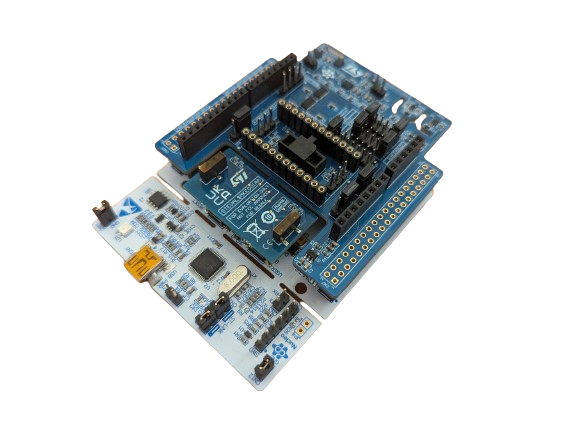
\includegraphics[scale=0.6]{../images/0002 nucleo-f411re.png}{\\STMicroelectronis NUCLEO-F411RE Mikrocontrollerboard mit X-NUCLEO-IKS4A1 Sensorboard}
\end{center}
Die Beschaffung aller Teile lief, bis auf ein überdimensioniertes Kabel und unterdimensioniert Propeller und Motoren reibungslos.\\
Allerdings war der ST NUCELO-F411RE nicht die erste Wahl. Zunächst wurde ein STM32-F4-DISCO bestellt. Da mit diesem aber keine serielle Verbindung zum Rechner aufgebaut werden konnte hatte das NUCLEO-F411RE Board die Möglichkeit sich, als würdigen Ersatz zu präsentieren. Dieser Fehler ist nicht als Beschaffungsfehler klassifiziert, sondern als Produktfehler.
\subsection{Rahmenproduktion}
Neben den Empfehlungen aus \ref{Beschaffung} hat sich auch herauskristallisiert, dass es hilft Teile zu haben, welche adaptiv sind. Der gewählte Rahmen wurde mit Teilen aus einem Baukasten der Firma Totem produziert, welche flexibel sind. Beispielsweise konnte die Rahmengeometrie oder -stärke schnell und ohne Beschaffungskosten angepasst werden. Technisch gesehen muss der Rahmen also nicht als Elementarteil, sondern schon als Produkt bezeichnet werden.
\subsection{Montierung und Anbindung der BLDC-Motoren und Treiber}
Die mechanische Schnittstelle zwischen dem Rahmen und den BLDC-Motoren muss mindestens alle nominal auftretenden Impulsströme leiten können. Nominale Zustände sind solche die beim Flug mit bis zu 30m/s und Starts- und Landungen mit bis zu 0.5m/s auftreten.\\
Die Verbindung wurde realisiert mit Bauteilen und 3mm-Schrauben aus dem Totem-Baukasten. Das Anlegen von Kraft orthogonal zum Rahmenarm offenbarte, dass die Verbindung zwischen Motor und Rahmen solide ist. Auch deutlich wurde aber, dass der Rahmen in ebendiese Richtung vergleichsweise leicht biegsam ist. Um dem entgegenzuwirken wurden für den zweiten Prototypen Querverstrebungen angeschraubt. Das Problem konnte dadurch gelöst werden zum Preis von etwas mehr Gewicht.

\subsection{\label{software:Software}Entwicklung der Simulations- und Lernsoftware}
\subsubsection{Analyse und Adaption der Quadcopterdynamik}
Die Simulationssoftware welche für die Reglerentwicklung wurde so ausgewählt und in Teilen entwickelt, dass Sie mit beliebigen Parameter funktioniert. Die Informatinen aus den vorangegangen Kapiteln mussten also nicht vorliegen für die Entwicklung der Simulationssoftware. Die folgenden Parameter sind jene die für den Großteil der Simulationen verwendet wurden. Ein wichtiger offener Punkt ist nach wie vor die Angleichung der Parameter an den Prototypen, sowie die Simulation und das Training von Reglern mit den realen Parameter. Anschließend kann die Kompatiblität des Modells zum Quadcoptersystem getestet werden. Offen geblieben sind die Punkte, da der Fokus auf der Entwicklung anderer System lag und das Training der PID-Parameter nicht wie Anfangs erwartet in einem Monat abgeschlossen werden konnte.
\vspace*{0.5cm}
\begin{center}
\begin{tabular}[h]{|l|l|l|l|l|}
\hline 
System & Komponenten & Modellparameter & Wert & Quelle \\
\hline 
Gesamt & Quadcopter & $m$ & $\approx $0.94kg & \\
& & $I_{B,xx}$ & 1.23e-2$\frac{kg}{m^2}$ & \ref{link:SimCon}\\
& & $I_{B,yy}$ & 1.23e-2$\frac{kg}{m^2}$ & \ref{link:SimCon}\\
& & $I_{B,zz}$ & 2.24e-2$\frac{kg}{m^2}$ & \ref{link:SimCon}\\
\hline
Impulsfluss & Propeller, Motor & $\tau$ & 0.1 & \ref{link:SimCon}\\
& & d & 1 (Keine Dämpfung)  & \ref{link:SimCon} \\
& & $k_p$ & 1 & \ref{link:SimCon} \\
& & $k_{Th}$ & 1.076e-5$\frac{Ns^2}{rad^2}$ & \ref{link:SimCon}\\
& & $k_{To}$ & 1.632e-7$\frac{Nms^2}{rad^2}$ & \ref{link:SimCon}\\
& Rahmen & $l$ & 0.25m & \\
& & $w$ & 0.25m & \\
& & $h_M$ & 0.05m & \\
\hline
Energiefluss & Akkumulator & $u_{max}$ & 7.4V & \ref{Akku}\\
& & $i_{max}$ & 40A & \ref{Akku}\\
& BLDC-Treiber & $u_{soll, gelb}$ & PWM(60Hz, 80\%-90\%) & \ref{link:Treiberdatenblatt}\\
& & $u_{soll, rot}$ & 5V & \ref{link:Treiberdatenblatt}\\
& & $u_{soll, braun}$ & 0V & \ref{link:Treiberdatenblatt}\\
\hline
\end{tabular}
\end{center}
\vspace*{0.5cm}
Für das Anlernen von Strategien sind dynamische Simulationen der Umwelt unabdingbar. Funktionen zur Quadcopterdynamiksimulation wurden aus dem Repository von John Bobzwik \ref{simcon:simcon} übernommen, wobei darauf zu achten war, dass die beigefügte Lizenz den Einsatz erlaubt.\\
Die Methode \textit{update} berechnet den nächsten Zustandsvektor des Quadcopters bei der in \textit{config.py} definierten Schrittweite. Der Vektor Zustand entspricht dem Zustandsvektor \ref{zustandsvektor:zustandsvektor} und in jedem Schritt aktualisiert. 
\begin{center}
\begin{tikzpicture}[font=\sffamily,every label/.append
style={font=\small\sffamily,align=center}]

\node[doc, fill=white] (Quadcontroller) {quad.py\\  \begin{lstlisting}[language=Python, basicstyle=\fontsize{8}{10}\selectfont]
...
def zustandsaenderung(self, t, zustand, motorbefehle, wind):
...

	# Differenzialgleichungen
	wddotM1 = (
		-2.0 * self.damp * self.tau * wdotM1 - 
		wM1 + 
		self.kp * motorbefehle[0]
	) / (self.tau ** 2)
	...
	
	wMotor = numpy.array([wM1, wM2, wM3, wM4])
	wMotor = numpy.clip(
		wMotor, 
		self.minWmotor, 
		self.maxWmotor
	)
	schub = self.kTh * wMotor * wMotor
	drehmoment = self.kTo * wMotor * wMotor
	
	# Inertialtensor
	IBxx = self.IB[0, 0]
	IByy = self.IB[1, 1]
	IBzz = self.IB[2, 2]
	
	MM * sdotn = RHS
	sdot = inv(MM) * RHS
	
	# Schrieben von wddot in sdot
	...
	
	self.beschleunigung = sdot[7:10]
	
	return sdot

def update(self, t, cmd, wind):
	geschwindigkeit_t_minus_1 = self.zustand[7:10]
	omega_t_minus_1 = self.zustand[10:13]
	
	self.integrator.set_f_params(cmd, wind)
	self.zustand = self.integrator.integrate(
		t, 
		t + config.Schrittweite
	)
	
	self.pos = self.zustand[0:3]
	self.quat = self.zustand[3:7]
	self.geschwindigkeit = self.zustand[7:10]
	self.omega = self.zustand[10:13]
	self.wMotor = numpy.array([
		self.zustand[13], 
		self.zustand[15], 
		self.zustand[17],
		self.zustand[19]
	])
	
	self.vel_dot = (
		self.geschwindigkeit - geschwindigkeit_t_minus_1
	) / config.Schrittweite
	self.omega_dot = (
		self.omega - omega_t_minus_1
	) / config.Schrittweite
	
	...
...
\end{lstlisting}
};
\end{tikzpicture}
\end{center}
Die Methode \textit{update} berechnet aus den Motorbefehlen, welche in der Einheit $rad/s$ vorliegen und optionalen Windparametern den nächsten Zustand.

\subsubsection{Architektur}
Zum Erreichen des Ziels der Quadcopterentwicklung wurden eine Reihe an lose gekoppelten Softwareanwendungen, welche teilweise autonom aber auch als Verbund operieren können, programmiert. In einem Repository Quadstar sind alle Daten und Programme zusammengefasst.
\begin{center}
	\begin{tikzpicture}[font=\sffamily,every label/.append
		style={font=\small\sffamily,align=center}]
		
		\node[doc, fill=white] (Quadcontroller) {./Quadstar/\\  \begin{lstlisting}[language=Python, basicstyle=\fontsize{8}{10}\selectfont] 
Modelle    
config.py       
joystick.py  
quaternion.py      
quad.py       
quadpid.py
quadendezuende.py       
quadlive.py  
quadtest.py        
quadregler.py  
quadseriell.py  
quadtrain.py  
wind.py    
			\end{lstlisting}
		};
	\end{tikzpicture}
\end{center}
Die Programmbeziehungen wurden visuell aufbereitet.
\begin{center}
	\begin{tikzpicture}[font=\sffamily,every label/.append
		style={font=\small\sffamily,align=center}]
		
		\node[doc, fill=green] at (-2, 1) (Quad) {quad.py};
		
		\node[doc, fill=green] at (-2, 3) (Quadlive) {quadlive.py};
		
		\node[doc, fill=green] at (-1, 5) (Quadtest) {quadtest.py};
		
		\node[doc, fill=green] at (-1, -1) (Quadserial) {quadserial.py};
		
		\node[doc, fill=green] at (2, 6) 
		 (Quadcontroller) {quadcontroller.py};

		\node[doc, fill=green] at (6, 3) (Quadmodel) {quadendezuende.py};

		\node[doc, fill=green] at (5, 5) (Quadpid) {quadpid.py};
		
		\node[doc, fill=blue!50] at (10, -2) (Quadsoft) {quadsoft.c};

		\node[doc,fill=blue!50] at (6, -7) (quadsoft) {quadsoft};

		\node[doc, fill=green, minimum width=2cm,minimum height=1cm] at (6, 1) (Config) {config.py};

		\node[doc, fill=green, minimum width=2cm,minimum height=1cm] at (5, -1) (Joystick) {joystick.py};

		\node[doc, fill=green, minimum width=2cm,minimum height=1cm] at (2, -2) (Quaternion) {quaternion.py};
		
		\draw[-latex] (Config.west) .. controls +(left:7mm) and +(left:7mm) .. (Quadpid.west);

		\draw[-latex] (Config.west) .. controls +(left:7mm) and +(left:7mm) .. (Quadmodel.west);

		\draw[-latex] (Config.west) .. controls +(left:7mm) and +(right:7mm) .. (Quadtest.east);

		\draw[-latex] (Config.west) .. controls +(left:7mm) and +(right:7mm) .. (Quad.east);

		\draw[-latex] (Config.west) .. controls +(left:7mm) and +(left:7mm) .. (Joystick.west);

		\draw[-latex] (Quadserial.east) .. controls +(right:7mm) and +(left:7mm) .. (Joystick.west);

		\draw[-latex] (Config.west) .. controls +(left:7mm) and +(right:7mm) .. (Quadserial.east);

		\draw[-latex] (Quad.east) .. controls +(right:7mm) and +(left:7mm) .. (Quadpid.west);

		\draw[-latex] (Config.west) .. controls +(left:7mm) and +(right:7mm) .. (Quadlive.east);

		\draw[-latex] (Quaternion.north) .. controls +(up:7mm) and +(right:7mm) .. (Quadlive.east);

		\draw[-latex] (Quadserial.east) .. controls +(right:7mm) and +(right:7mm) .. (Quadlive.east);

		\draw[-latex] (Quaternion.north) .. controls +(up:7mm) and +(right:7mm) .. (Quadtest.east);

		\draw[-latex] (Quad.east) .. controls +(right:7mm) and +(right:7mm) .. (Quadtest.east);

		\draw[-latex] (Quad.east) .. controls +(right:7mm) and +(left:7mm) .. (Quadmodel.west);

		\draw[-latex] (Quaternion.north) .. controls +(up:7mm) and +(left:7mm) .. (Quadmodel.west);

		\draw[-latex] (Quaternion.north) .. controls +(up:7mm) and +(right:7mm) .. (Quad.east);

		\draw[-latex] (Quadcontroller.south) .. controls +(down:7mm) and +(right:7mm) .. (Quadtest.east);

		\draw[-latex] (Quaternion.north) .. controls +(up:7mm) and +(left:7mm) .. (Quadpid.west);

		\draw[-latex, dash pattern=on 10pt off 5pt] (Quadserial.south) .. controls +(down:25mm) and +(up:20mm) .. (quadsoft.north) node[midway, left,font=\small\sffamily]{Sollgeschwindigkeit};

		\draw[-latex, dash pattern=on 10pt off 5pt] (Quadsoft.south) .. controls +(down:20mm) and +(up:20mm) .. (quadsoft.north);

		\draw[-latex] (Quad.east) .. controls +(right:7mm) and +(right:7mm) .. (Quadlive.east);
		
		\node[draw,dashed,rounded corners,fit=(Quadsoft),inner
		xsep=10pt,inner ysep=30pt,label={above:{STM32CubeIDE}}](fit3){};

		\node[draw,dashed,rounded corners,fit=(Quadlive) (Quadtest) (Quadserial) (Quadcontroller) (Quadmodel) (Quadpid) (Quaternion) (Quad) (Config),inner
		xsep=10pt,inner ysep=30pt,label={above:{Visual Studio Code}}](fit4){};

		\node[draw,dashed,rounded corners,fit=(fit3) (fit4),inner
		xsep=10pt,inner ysep=30pt,label={above:{Thinkpad P52s}}](fit4){};
		
		\node[parallelepiped,draw=yellow,fill=red!80,
		minimum width=2cm,minimum height=1.5cm,align=center,text=white] at (0, -7) (imu) {IMU};
		
		\node[right=1.5cm of quadsoft, doc, fill=yellow, minimum width=2cm, minimum height=1cm] (HTML) {PWM, CCR};
		
		\draw[-latex] (imu) -- (quadsoft) node[midway, above, font=\small\sffamily]{Messwerte};
		
		\draw[-latex] (quadsoft) -- (HTML) node[midway, below, font=\small\sffamily]{Befehle};
		
		\draw[-latex, dash pattern=on 10pt off 5pt] (quadsoft.north) .. controls +(up:25mm) and +(down:20mm) .. (Quadserial.south) node[midway, right,font=\small\sffamily]{Messwerte};
		
		\draw[-latex] (Quad.east) .. controls +(right:7mm) and +(down:7mm) .. (Quadcontroller.south) node[midway, right, font=\small\sffamily]{};
		
		\node[draw,dashed,rounded corners,fit=(quadsoft) (HTML),inner
		sep=10pt,label={above:{NUCLEO-F411RE}}](fit4){};
		
		\node[draw,dashed,rounded corners,fit=(imu),inner
		sep=10pt,label={above:{X-NUCLEO-IKS4A1}}](fit5){};
		
	\end{tikzpicture}
\end{center}
Alle Python Dateien enthalten eine Klasse und instanziieren mindestens eine andere Klasse. Neben den Python Dateien welche mit Visual Studio Code entwickelt worden sind, wurde das Reglerprogramm mit C in der STM32CubeIDE geschrieben.
Das Diagramm visualisiert Klassen welche andere instanziieren und Informationsflüsse über eine serielle Schnittstelle mit Pfeilen. Ein Pfeil von einer Python Datei zu einer anderen bedeutet letztere Python Datei arbeitet mit erster. Gestrichelte Pfeil stellen Informationsfluss über UART dar.\\
Die in \textit{quad.py} definierte Klasse Quadcopter umfasst vor allem die Quadcopterdynamiksimulation \ref{simcon:simcon}. Mit \textit{quadtrain.py} welche Methoden aus \textit{quadpid.py} oder \textit{quadendezuende.py} aufruft lassen sich PID-Parameter beziehungsweise Ende-zu-Ende-Modelle lernen. 
Die Klassen \textit{Quadpid} und \textit{Quadendezuende} welche in \textit{quadpid.py} beziehungsweise \textit{quadendezuende.py} definiert sind erben von \text{gym.Env} \ref{gymnasium} und implementierten die Funktionen \textit{reset} und \textit{step}. Trainiert der Nutzer ein Modell mit \textit{quadtrain.py} greift Stable Baselines3 auf eine der Umwelten zu entsprechend der Definition in \textit{config.py}. Weiterführende Details zur Implementierung, Spezifizierung und zu den Hyperparametern der Trainingsumgebungen werden in \ref{pidlernen} und \ref{EndeZuEndeModell}\\ vorgestellt. Durch den Aufruf von \textit{quadlive.py} wird ein Flask-Server gestartet mithilfe von welchem die Trajektorie eines Quadcopter im Browser simuliert wird. 
\begin{center}
	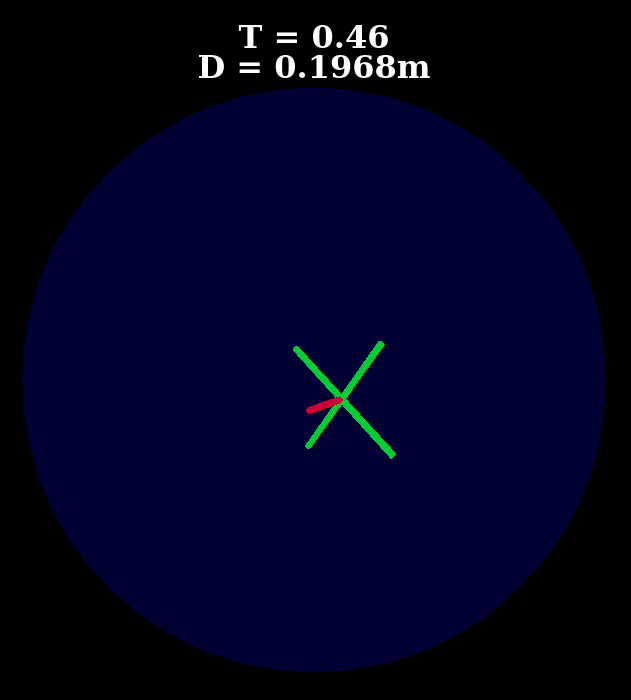
\includegraphics[scale=0.3]{../images/0068 Quadlive 1.png}{\\Visualisierung des Quadcopters mit \textit{quadlive.py} im Browser}
\end{center}
Die Webvisualisierung greift auf Methoden aus \textit{quadtest.py} zurück welche auch dazu verwendet werden können, Plots von Trajektorien zu erstellen. Gezeichnet werden 6 translatorischen Parameter welche die Position und Geschwindigkeit des Quadcopters im Nord-Ost-Unten Orientierungssystem repräsentieren und 3 rotatorische Parameter, welche die Drehlage darstellen, wobei die Darstellung in Polarkoordinaten gewählt wurde, um der periodischen Natur der Größe gerecht zu werden.\\
Die Entwicklung und Implementierung des Programms \textit{quadsoft.c}, auf dem NUCELO-F411RE Board, ist Teil des Arbeitsschrittes Reglerimplementierung \ref{Reglerimplementierung:Reglerimplementierung}.\\
Hervorzuheben ist die \textit{config.py} Datei, da in ihr alle relevant Parameter zum Einstellen des Programmverhaltens zusammengefasst sind. Daneben hat die Datei die Funktion Modellbeschreibungsdateien, welche beim Training in den Modellordner kopiert werden, zu leiten. Will der Nutzer ein trainiertes Modell testen kann er einfach die Konfigurationsdatei in das Hauptverzeichnis kopieren, wodurch das Programm dieses erkennt und anwendet, sofern der Nutzer keine Änderung an der Bezeichnung vorgenommen hat. In Zukunft ist denkbar, die Configuration kann vom Nutzer wegzuabstrahieren wodurch allerdings potenziell eine Freiheitseinschränkung mit einhergehen könnte. Die wichtigsten Parameter werden kurz beschreiben.
\vspace*{0.5cm}
\begin{center}
	\begin{tabular}[h]{|c|c|c|c|}
		\hline 
		Konfigurationsparameter & Typischer Wert & Bedeutung\\
		\hline
		Umweltparameter & & \\
		Schrittweite & 1e-3 & Schrittweite in s\\
		Finaler Zeitpunkt & 1s & Simulationsende in s\\
		Initaler Zeitpunkt & 0s & Simulationsbeginn in s\\
		\hline 
		Quadtrain & & \\
		Ordnername & QM-01-01-2024-SC42-A & Modellordner\\ 
		Episoden & 1e8 & Episodengesamtzahl \\
		Actor & [2, 2] & Schichtentopologie Actor\\
		Critic & [2, 2] & Schichtentopologie Critic\\ 
		Lernrate ($\alpha$) & 1e-4 & Lernrate \\
		Parallele Umwelten & 4 & siehe \ref{paralleleUmwelten}\\
		Batchmenge & 16 & Batchmenge\\
		\hline 
		Quadendezuende & &\\
		Aktionsraum Datentyp & float32 &\\
		Aktionsraum EndeZuEnde & [0$\frac{rad}{s}$ bis 1000$\frac{rad}{s}$] & siehe \ref{EndeZuEndeModell}\\
		Belohnungsgewichtung & [0.0, 0.4, 0.2, 0.4] & siehe \ref{Belohnung}\\
		\hline
	\end{tabular}
\end{center}
Der Ordnername, im Beispiel QM-01-01-2024-SC42-1, setzt sich zusammen aus einem Reglerbezeichner, dem Datum im Format Tag, Monat und Jahr, einem Hardwarebezeichner und abschließend einer Identifikationsnummer. Der Reglerbezeichner QM steht für Ende-zu-Ende-Modelle. PID-Regler wurden mit QP bezeichnet. Das Datum markiert den Tag, an dem mit dem Training des Modells begonnen wurde und der Identifikationsbuchstabe unterscheidet Modelle eines Tages, sodass diese bei Modellen mit unterschiedlichem Datum dieselbe sein kann.

\subsubsection{\label{Belohnung}Belohnungsfunktionen}
Die Belohnungsfunktion ist inspieriert von \ref{link:ReinforcementLearningQuadcopter}. \\
Der Nutzer kann vier Belohnungsfunktionen gewichten.
Diese berechnen die Belohnung positionsbasiert
\begin{align}
r_p(x, y, z) &= \frac{1}{1 + (x - x_{soll})^2 + (y - y_{soll})^2 + (z - z_{soll})^2}
\end{align}
lagebasiert
\begin{align}
r_{\varphi}(\phi, \theta, \psi) &= \frac{1}{1 + (\phi - \phi_{soll})^2 + (\theta - \theta_{soll})^2 + (\psi - \psi_{soll})^2}
\end{align}
geschwindigkeitsbasiert
\begin{align}
r_v(v_{N}, v_{O}, v_{U}) &= \frac{1}{1 + (v_{N} - v_{N, soll})^2 + (v_{O} - v_{O, soll})^2 + (v_{U} - v_{U, soll})^2}
\end{align}
und drehratenbasiert
\begin{align}
r_{\dot{\varphi}}(\dot{\phi}_x, \dot{\theta}_y, \dot{\psi}_z) &= \frac{1}{1 + (\dot{\phi} - \dot{\phi}_{soll})^2 + (\dot{\theta} - \dot{\theta}_{soll})^2 + (\dot{\psi} - \dot{\psi}_{soll})^2}.
\end{align}
Die Gewichtung erfolgt mit 4 Parametern 
\begin{align}
r &= \alpha_r r_p + \beta_r r_v + \gamma_r r_{\varphi} + \delta_r r_{\dot{\varphi}}.
\end{align}
Die Summe der Parameter
\begin{align}
\alpha_r + \beta_r + \gamma_r + \delta_r &= 1 
\end{align}
sollte immer Eins sein um Vergleichbarkeit herzustellen.
Die Autoren von \ref{link:ReinforcementLearningQuadcopter} beobachteten eine starke Abhängigkeit der Lernperformance von der Wahl der Parameter. Da für den Quadcopter ein Geschwindigkeitsregler implementiert werden soll, spielt die Positionsbelohnung $r_p$ nur eine untergeordnete Rolle.\\
Bei der vorgestellten Belohnungsfunktion handelt es sich nicht um die einzige verwendete.

\subsubsection{Beobachtungsraum}
Die Beobachtung enthält die Ist- und die Sollgeschwindigkeit sowie die Drehlage, welche aus der Quaternionen des Zustandsvektors $s$ berechnet wird. Zunächst wurde der Beobachtungsraum ohne die Istgeschwindigkeit aufgestellt. Da mit diesem Setup kein Modell lernte wurde Sie testweise hinzugenommen und praktisch ein Problem aus dem Bereich des Überwachten Lernens \ref{link:MaschinellesLernen} zu einem des Tiefen Verstärken Lernens gemacht. Ob das Sinnvoll ist wird nicht weiter elaboriert. Mit dem Setup gelang es aber zumindest kleine Lernerfolge \ref{EndeZuEndeModell} mit Tiefen Verstärkendem Lernen zu erzielen.
\begin{align}
	s_t &= \begin{pmatrix}
		v_3\\
		v_{3, Soll}\\
		\varphi_3
	\end{pmatrix}
\end{align}
In der Simulation werden die Werte für alle Beobachtungen direkt aus dem Zustandsvektor ausgelesen. Bedeutet es wurde kein Sensorrauschen simuliert und auch das Übertragungsverhalten der Sensoren wurde nicht betrachtet. 

\subsubsection{\label{Geschwindigkeitssollvektor}Geschwindigkeitssollvektor}
Der Geschwindigkeitssollvektor welcher für das Training aller PID und Ende-zu-Ende Modelle eingesetzt wurde, enthält 8 Elemente und ermöglicht keine Bewegung auf der Unten-Dimension. Die Unten-Dimension wurde ignoriert da das Lernen von acht Sollgeschwindigkeiten als einfacher erachtet wurde als das Lernen von 27 Dimension.
\begin{align}
	v_{Soll} &= \begin{pmatrix}
		\text{randint}(-1, +1)\\
		\text{randint}(-1, +1)\\
		0
	\end{pmatrix}
\end{align}
Auch mit einem Joystick wurden Sollwerte produziert, als Teil der Testbench \ref{testbench:testbench}. Die zwei Sollwertinterface funktionieren unabhängig voneinander. Wichtig ist nur, dass das Format für das Training dem Format des Quadcopterreglers auf dem Mikrocontroller entspricht.
Im Laufe der Entwicklung unterlief der Geschwindigkeitssollvektor kontinuierlich Anpassungen. Gewählt wurde die Form da Sie auf die Zustände eines Joysticks, ohne Schub passt. Ein Durchdrücken des Joysticks nach vorne rechts entspricht dem Geschwindigkeitssollvektor
\begin{align}
	v_{Soll,Vorne,Rechts} &= \begin{pmatrix}
		1\\
		1\\
		0
	\end{pmatrix}.
\end{align}
Alle weiteren Joystickzustände ergeben sich entsprechend. 

\subsection{\label{pidlernen}Lernen der PID-Parameter}
Durch das Lernen von PID-Parameter kann in der Theorie sowohl die Reglerperformance maximiert werden als auch auf die manuelle Parametersuche verzichtet werden.\\
Das Anlernen des PID-Geschwindigkeitsregelers umfasste bis zu 18 PID-Parameter. Zu beachten ist, dass für die Nord- und Ost-Dimension häufig eine Aktion zwei Parameter bestimmt. Die tatsächliche Zahl der PID-Parameter im Geschwindigkeitsregler ist 24.
\begin{align}
	a_t &= \begin{pmatrix}
		P_{v,3}\\
		I_{v,3}\\
		D_{v,3}\\
		P_{q,3}\\
		P_{\varphi,3}\\
		P_{\dot{\varphi},3}\\
		D_{\dot{\varphi},3}
	\end{pmatrix}
	= \begin{pmatrix}
		P-Geschwindigkeit (Nord, Ost, Unten)\\
		I-Geschwindigkeit (Nord, Ost, Unten)\\
		D-Geschwindigkeit (Nord, Ost, Unten)\\
		P-Drehlage (Quaternion)\\
		P-Drehlage (Rollen, Nicken, Gieren)\\
		P-Drehrate (Rollrate, Nickrate, Gierrate)\\
		D-Drehrate (Rollrate, Nickrate, Gierrate)\\
	\end{pmatrix}
\end{align}
Der Regler berechnet zunächst mithilfe von PID-Geschwindigkeitsregelern einen Sollschubvektor. Dieser Sollschubvektor wird umgerechnet zu einer Solldrehlage welche in Quadternionenfrom Eingang für das Kontrollgesetz ist, vergleich \ref{Quadcopterregelungsproblem}.\\
Die Visualisierung zeigt ein Standard-Regelkreis welcher Teil der Gesamtarchitektur ist die den Regelkreis ergänzt um einen PPO-Agenten und eine Belohnungsfunktion. Verdeutlichen soll die Visualisierung nicht die Softwarearchitektur sondern den Unterschied zwischen der Schrittweite des Regelkreises $n_R$ und der Schrittweite bis der Agent $n_{PPO}$ neue PID-Parameter im PID-Regler setzt. Anfangs wurden verschiedene adaptive Regler trainiert, also solche mit 
\begin{align}
	n_{PPO}\Delta t_{Modell} < n_R\Delta t_{Modell}\cdot \text{Episodenende}
\end{align}
bei denen in einer Episode die PID-Parameter nicht nur einmal zu Beginn gesetzt werden. Spätestens als sich das Problem des Lernens von PID-Parameter als schwerer als erwartet erwiesen hat wurde nicht mehr an adaptiven, kombinierten PID-/PPO-Reglern geforscht. Die Parameter wurden in jeder Episode zu Beginn einmal gesetzt, was einem \textit{step} pro Episode in Famara Gymnasium entspricht.
\begin{center}
\begin{tikzpicture}[font=\sffamily, every label/.append style={font=\small\sffamily, align=center}]

\node[doc] (Regler) {PID-Regler};

\node[right=1cm of Regler, doc] (Umweltmodell) {
	Umweltmodell, $f_U$
};

\node[below=2.3cm of Regler, doc] (Observationsmodell) {
	Observationsmodell
};

\node[left=4cm of Regler, doc] (Sollwertinterface) {
	Sollwertinterface
};

\draw[-latex] (Regler) -- (Umweltmodell) node[above, midway, font=\small\sffamily]{$\omega_t$};

\node[left=2.5cm of Regler, circle, draw] (c) at (0,0) {-}; 

\draw[-latex] (Observationsmodell) -| (c) node[midway, left, font=\small\sffamily]{$s_{t, Mess}$};

\draw[-latex] (c) -- (Regler) node[above, midway, font=\small\sffamily]{$e_t$};

\draw[-latex] (Umweltmodell) |- (Observationsmodell) node[right, midway, font=\small\sffamily]{$y_t$};

\draw[-latex] (Sollwertinterface) -- (c) node[above, midway, font=\small\sffamily]{$s_{Soll}$};

\node[
draw,
dashed,
rounded corners,
fit=(Regler) (Umweltmodell) (Sollwertinterface) (Observationsmodell),
inner sep=10pt,
label={above:{Regelkreis}}
](fit5){};

\node[above=2.6cm of Regler, doc] (PPO) {PPO};

\node[above=1cm of PPO, doc] (Belohnungsfunktion) {Belohnungsfunktion};

\draw[-latex] (Umweltmodell) |- (PPO) node[right, midway, font=\small\sffamily]{$s_{t}$};

\draw[-latex] (Umweltmodell) |- (Belohnungsfunktion);

\draw[-latex] (Belohnungsfunktion) -- (PPO) node[right, midway, font=\small\sffamily]{$r_{t}$};

\draw[-latex] (PPO) -- (Regler)node[right, midway, font=\small\sffamily]{$a_{t}$};

\draw[-latex] (Sollwertinterface) |- (Belohnungsfunktion)node[left, midway, font=\small\sffamily]{$s_{Soll}$};

\node[
	draw,
	dashed,
	rounded corners,
	fit=(Regler) (Umweltmodell) (Sollwertinterface) (Observationsmodell) (PPO) (Belohnungsfunktion) (fit5),
	inner sep=10pt,
	label={above:{Architektur}}
](all2){};


\draw[-latex] (1.8, -1) arc (90:-220:0.8) node[above, font=\small\sffamily]{$f_{R}$};

\draw[-latex] (1.8, 3) arc (90:380:0.8) node[above, font=\small\sffamily]{$f_{PPO}$};

\end{tikzpicture}
\end{center}
\vspace*{0.5cm}
Da nicht auf alle trainierten Modelle eingengangen werden kann wird der Fokus auf den vielversprechensten liegen. Das erfolgversprechenste Modell für PID-Parameter hat die folgende Konfiguration und wurde für 220e3 Episoden trainiert. 
\begin{center}
\begin{tabular}[h]{|c|c|}
\hline 
Konfigurationsparameter & Wert \\
\hline 
Umweltparameter & \\
Schrittweite $\Delta t_{Modell}$ & 1e-3s \\
Episodenende & 1s\\
\hline
Quadtrain & \\
Ordnername & QP-12-09-24-EIPC55-A\\
Lernrate $\alpha$ & 1e-4\\
Parallele Umwelten & 4\\
Batch & 16\\
Netzwerktopologie $\pi$ & [2, 2]\\
Netzwerktopologie $V^{\pi}$ & [2, 2]\\
\hline
Quadendezuende & \\
Aktionsraum Datentyp & float32\\
Aktionsraum & [0 bis 10]\\
$\alpha_r$ & 0.0\\ 
$\beta_r$ & 0.6\\
$\gamma_r$ & 0.2\\
$\delta_r$ & 0.2\\
\hline
\end{tabular}
\end{center}
\vspace*{0.5cm}
Der Rechner EIPC55 hat 32GB RAM und eine Intel Xeon CPU die mit bei zu 3900MHZ taktet. Als GPU ist eine RTXA4000 verbaut.
\begin{center}
	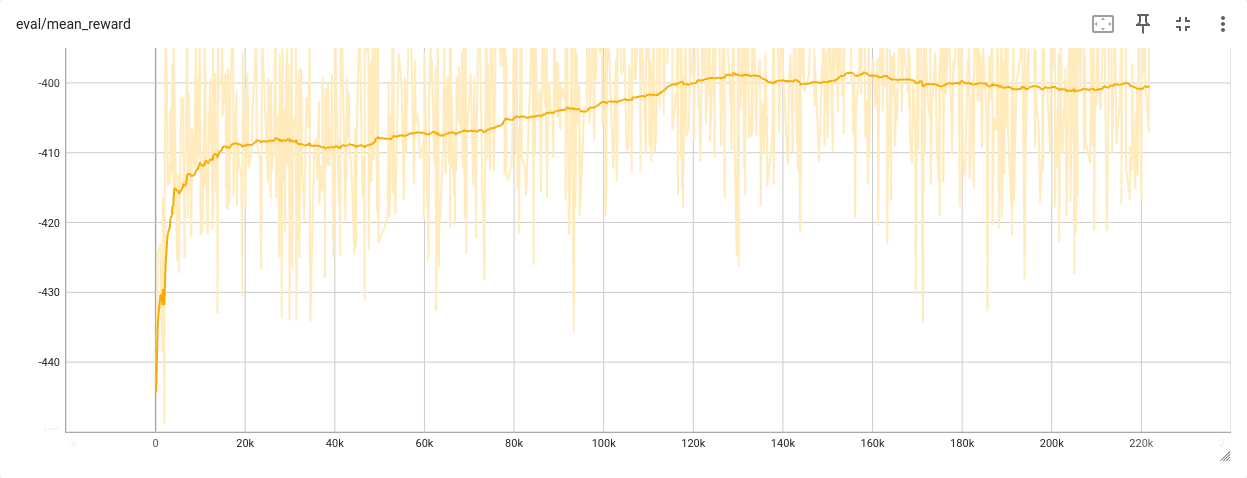
\includegraphics[scale=0.38]{../images/0089 PID Lernen.png}{\\Mittlerere Belohnung als Funktion der Episode aufgezeichnet und dargestellt mit Tensorboard. Wichtig ist das der Lernerfolg einsetzte nachdem die Belohnungsfunktion von der in \ref{Belohnung} abgewandelt wurde auf eine der From $-|e_v|$. In jedem Quadcopterschritt wird die Belohnung berechnet wie mit den vorgestellten Belohnungsfunktion \ref{Belohnung} und auf die Episodenbelohnung addiert, sodass nicht nur der Quadcopterschritt die Belohnung determiniert. Ob die veränderten Hyperparameter dieses Modell halbwegs akzeptabel lernen lassen haben oder tatsächlich die Belohnungsfunktion muss noch analysiert werden.}
\end{center}
\pagebreak 
Die Bilder zeigen exemplarisch, simulierte Positions-, Geschwindigkeits- und Drehlagetrajektorien in blau sowie Positions- und Geschwindigkeitssolltrajektorien in grün. Zunächst werden die Default PID-Parameter aus \ref{simcon:simcon} betrachtet.
\begin{center}
	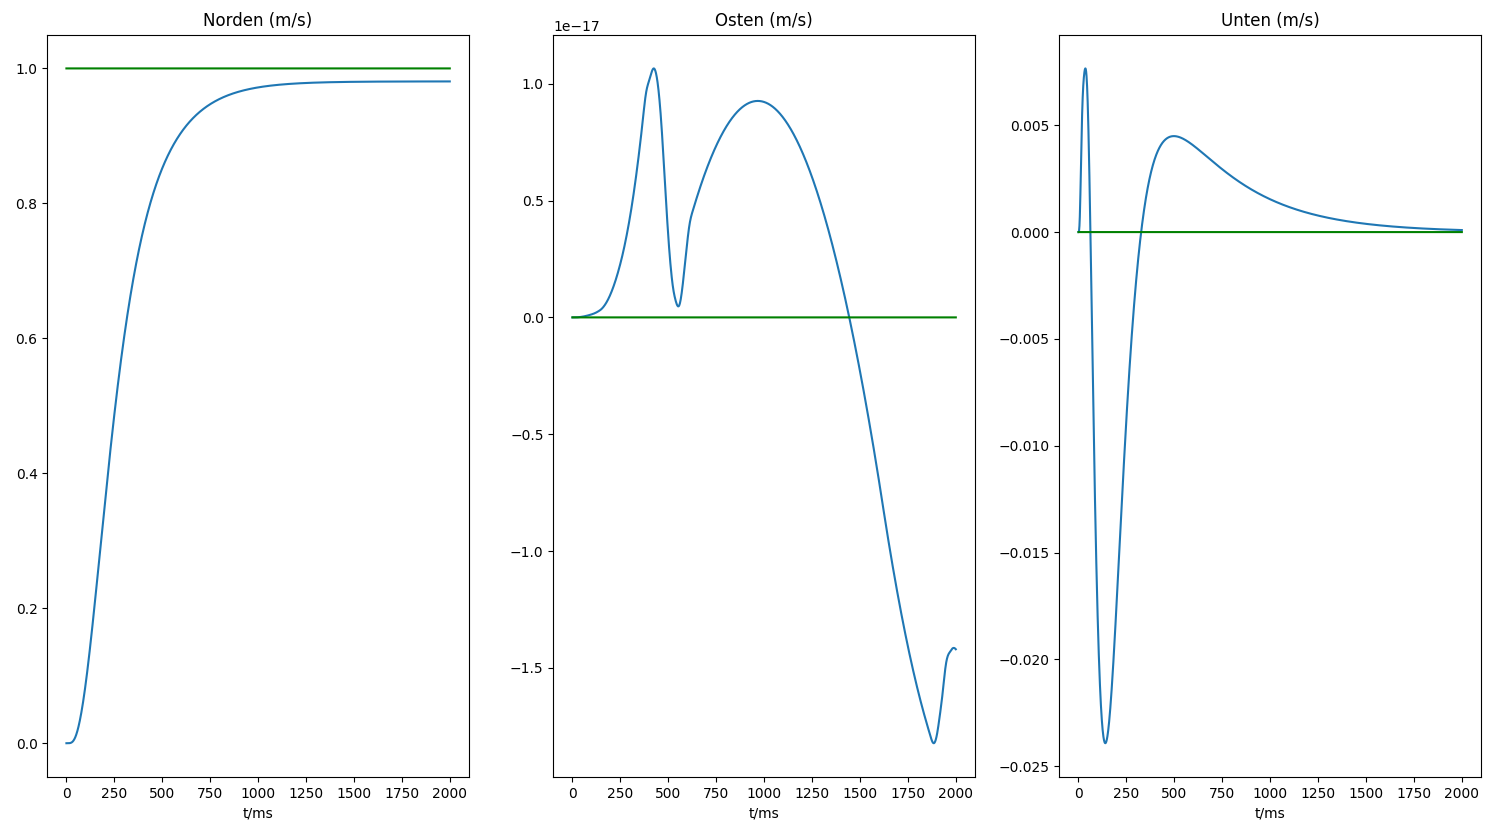
\includegraphics[scale=0.25]{../images/0096 Geschwindigkeit.png}{\\Die Istgeschwindigkeit folgt der Sollgeschwindigkeit in erster Näherung perfekt bis auf den unerwarteten verbleibenden Fehler auf der Nord-Dimension.}
\end{center}
\begin{center}
	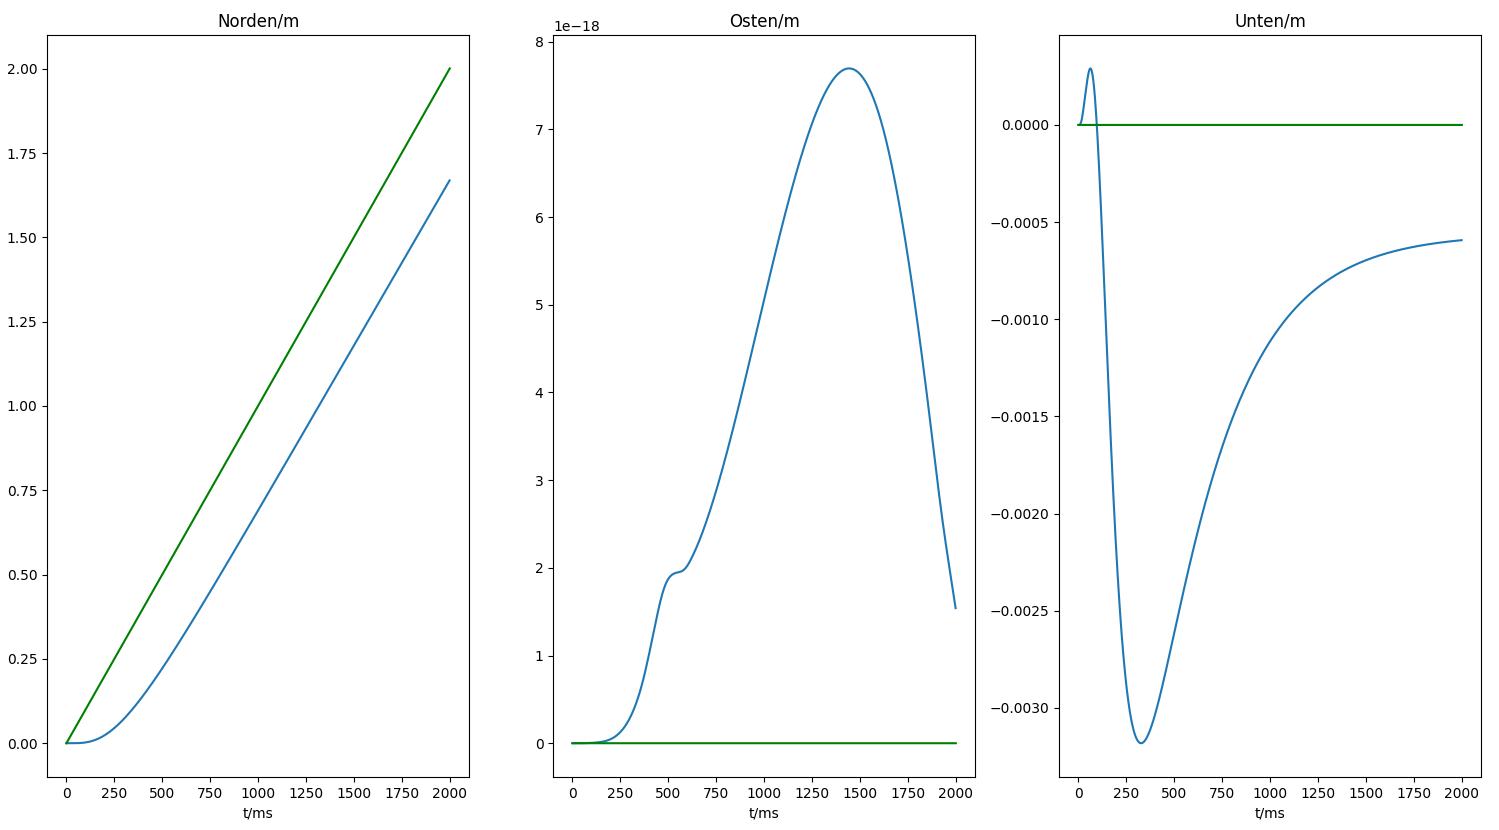
\includegraphics[scale=0.25]{../images/0098 Position.png}{\\Die Wirkung des verbleibenden Fehlers zwischen Ist- und Sollgeschwindigkeit ist im Positionsplot kaum sichbar da während der Beschleunigungsphase ein Offset entsteht.}
\end{center}
\begin{center}
	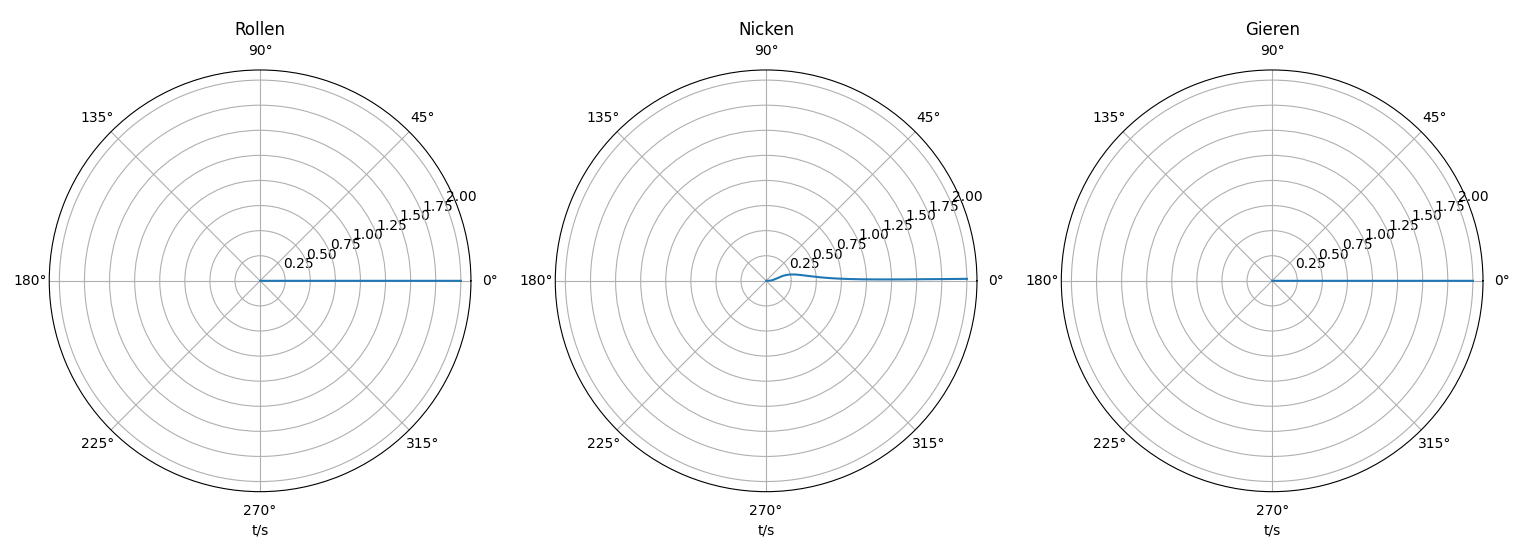
\includegraphics[scale=0.25]{../images/0097 Drehlage.png}{\\Winkel}
\end{center}
\pagebreak
Die Trajektorien ergeben sich wenn der PID-Regler mit gelernten Parametern arbeitet.
\begin{center}
	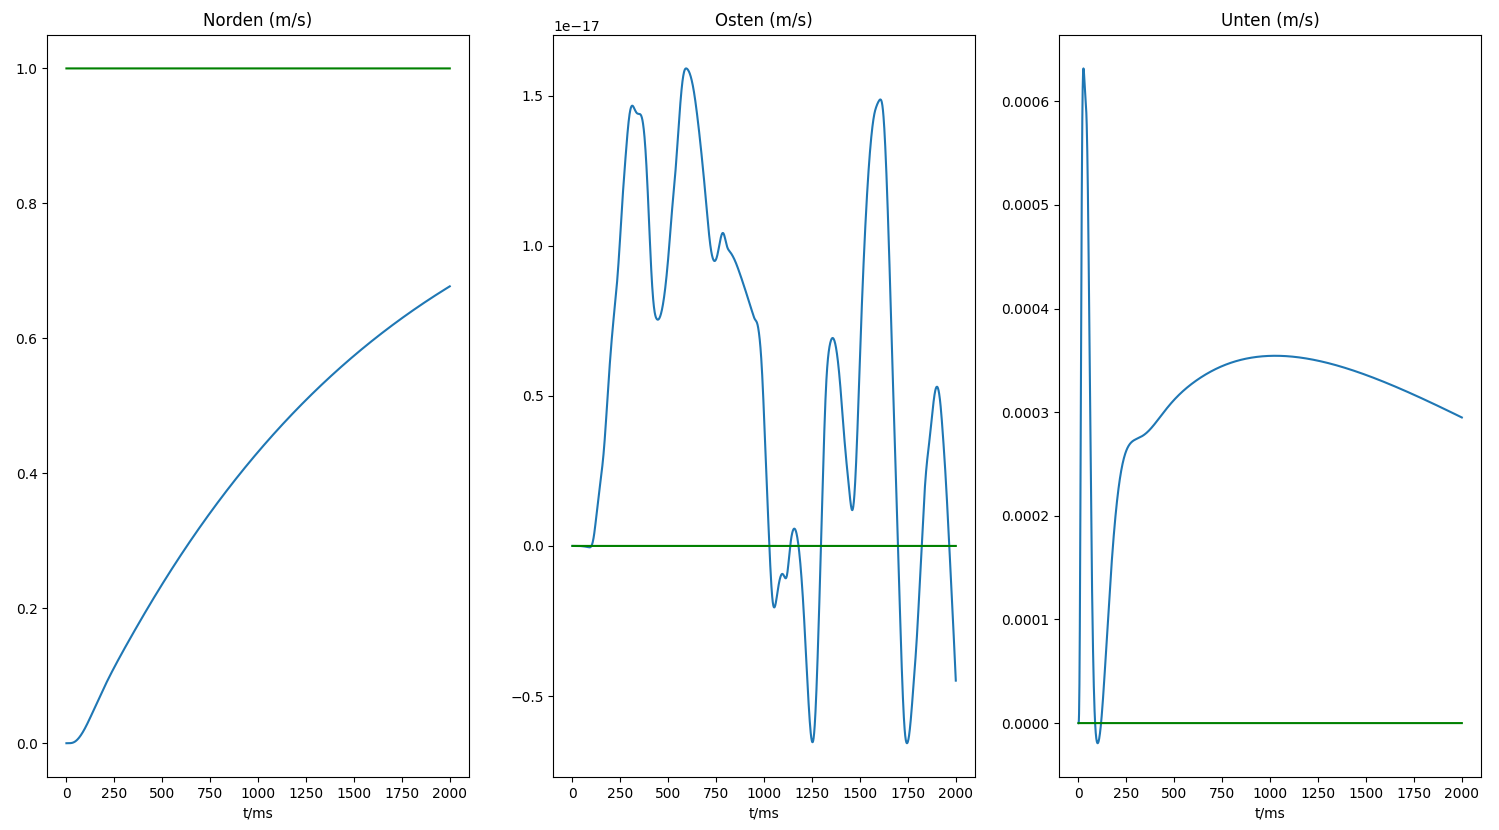
\includegraphics[scale=0.25]{../images/0093 Geschwindigkeit.png}{\\Die Parameter wurden gelernt sodass, der Regler gegen die Sollgeschwindigkeit konvergiert. Allerdings ist der gelernte PID-Regler grob abgeschätzt um den Faktor 4 mal später bei der halben Sollgeschwindigkeit.}
\end{center}
\begin{center}
	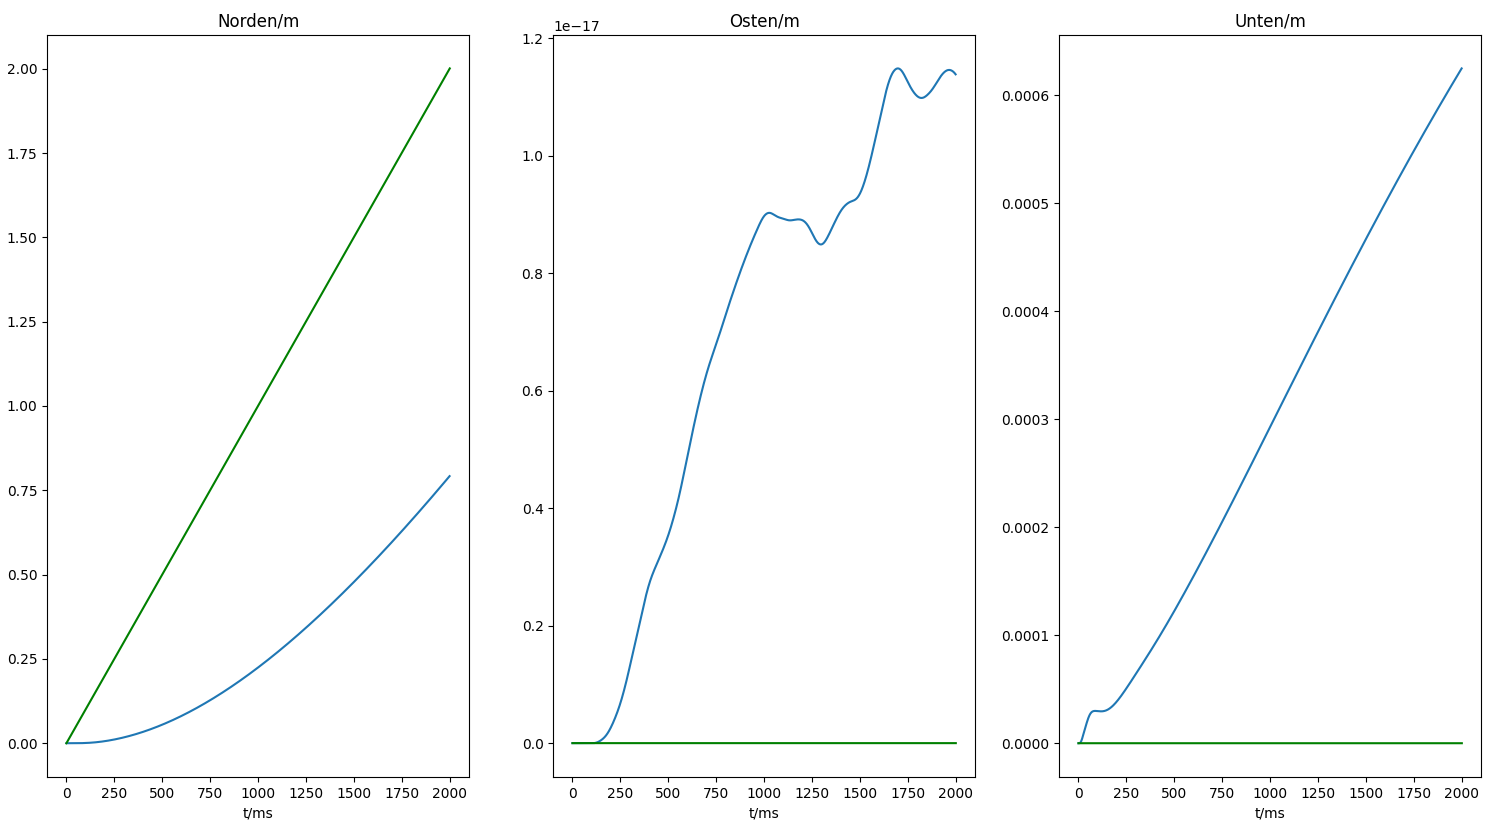
\includegraphics[scale=0.25]{../images/0094 Position.png}{\\Nach 2 Sekunden hat der Quadcopter noch keinen Meter zurückgelegt.}
\end{center}
\begin{center}
	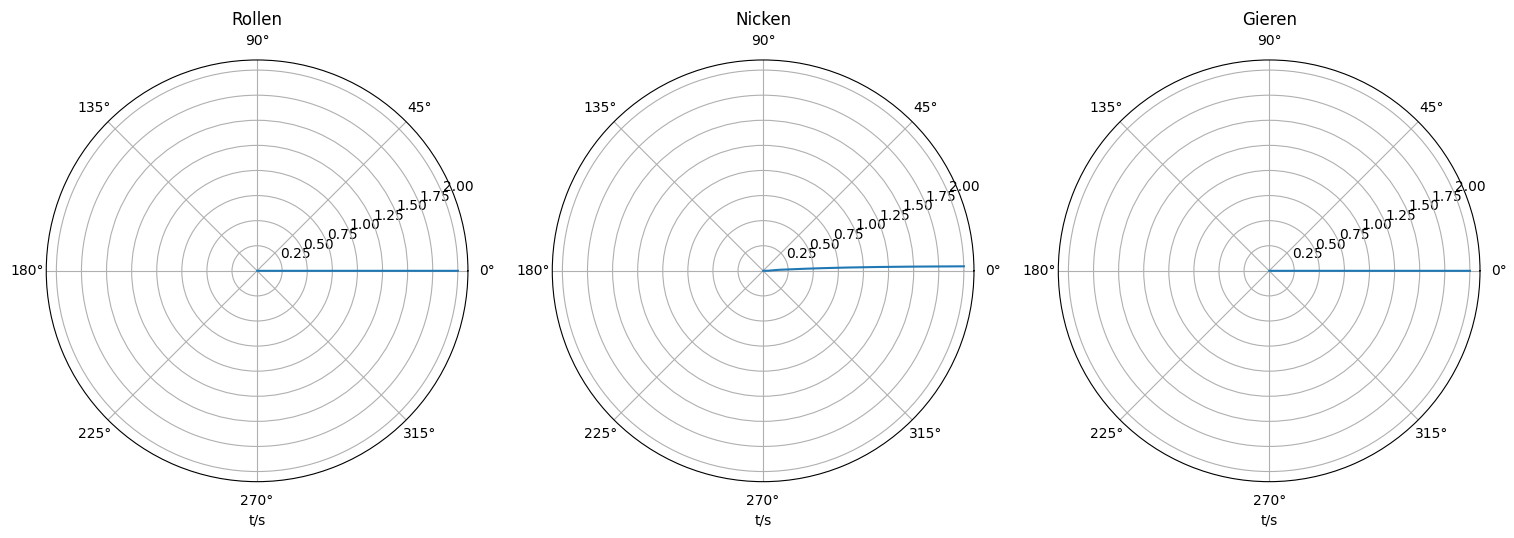
\includegraphics[scale=0.25]{../images/0095 Drehlage.png}{\\Der Quadcopter nickt deutlich schwächer.}
\end{center}
Die Herausforderung beim Lernen der PID-Parameter für den Geschwindigkeitsregler war Belohnungsfunktionen zu entwerfen die mit geringer Belohnungsvarianz und kontinuirlichen\\ Beobachtungs- und Aktionsräumen umgehen können. PID-Parameter Optimierung scheint ein stärker nichtkonvexes Problem zu sein als zunächst erwartet. Da nur einmal am Anfang pro Episode eine Aktion ausgeführt und eine Belohnung erfahren wird ist zudem die Sampleeffizient besonders gering. Die Kombination aus gewaltigem Quadcopterzustandsraum und Nichtlinearität verstärken den Fluch der Dimensionalität. Die Actor-Critic Architektur addressiert unter anderem das Problem der Sampleineffizienz scheint aber noch kein Allheilmittel zu sein. Grob geschätzt ist anzunehmen, dass nach einem Monat Training auf der vorliegenden Hardware alle Reglerparameter auf einen hohes Güteniveu gebracht werden können. Validieren lässt sich diese Aussage nur durch weiteres Training.

\subsection{\label{EndeZuEndeModell}Lernen des Ende-zu-Ende-Modells}
Ziel des Ende-zu-Ende-Lernens war mit PPO einen Agenten zu trainieren, welcher aus der Beobachtung bestimmter Quadcopterzustände direkt Motorbefehle vorhersagt, sodass die Quadcoptergeschwindigkeit so minimal wie möglich vom Geschwindigkeitssollvektor abweicht \ref{Geschwindigkeitssollvektor}. Der Aktionsraum besteht dementsprechend aus den vier Motorbefehlen.
\begin{align}
a_t &= 
\begin{pmatrix}
	u_{M1}\\
	u_{M2}\\
	u_{M3}\\
	u_{M4}
\end{pmatrix}
\end{align}
In \ref{link:ReinforcementLearningQuadcopter} wird auf ähnliche Weise versucht ein gleichwertiges Ziel zu erreichen.\\
Die Architektur für das Lernen des Ende-zu-Ende-Modells reduziert sich im Vergleich zur PID-Architektur auf das Umweltmodell, das Sollwertinterface, die Belohnungsfunktion und den Algorithmus des verstärkenden Lernens. Das Umweltmodell unterscheidet sich nur an den Schnittstellen zu dem aus der PID-Implementierung. Als Algorithmus wurde erneut Proximal-Policy-Optimization angewendet.
\begin{center}
\begin{tikzpicture}[
font=\sffamily, every label/.append style={font=\small\sffamily, align=center}]
\node[doc] (PPO) {PPO};

\node[below right=2cm of PPO, doc] (Umweltmodell) {Umweltmodell, $f_U$};

\node[above=1cm of PPO, doc] (Belohnungsfunktion) {Belohnungsfunktion};

\node[left=2cm of Belohnungsfunktion, doc] (Sollwertinterface) {Sollwertinterface};

\draw[-latex] (Umweltmodell) |- (PPO) node[right, midway, font=\small\sffamily]{$s_{t}$};

\draw[-latex] (Umweltmodell) |- (Belohnungsfunktion);

\draw[-latex] (Belohnungsfunktion) -- (PPO) node[right, midway, font=\small\sffamily]{$r_{t}$};

\draw[-latex] (Sollwertinterface) -- (Belohnungsfunktion) node[midway, above, font=\small\sffamily]{$s_{Soll}$};

\draw[-latex] (Sollwertinterface) |- (PPO) node[midway, left, font=\small\sffamily]{$s_{Soll}$};

\draw[-latex] (PPO) |- (Umweltmodell) node[left, midway, font=\small\sffamily]{$a_{t}$};

\node[
draw,
dashed,
rounded corners,
fit=(Regler) (Umweltmodell) (Sollwertinterface) (PPO) (Belohnungsfunktion),
inner sep=10pt,
label={above:{Architektur}}
](all2){};

\draw[-latex] (1.8, -0.2) arc (90:380:0.8) node[above, font=\small\sffamily]{$f_{PPO}$};

\end{tikzpicture}
\end{center}
Nach über 3e7 Episoden zeigte der Algorithmus keine Anzeichen von Belohnungsgewinnen und auch Änderungen der Hyperparameter zeigten keine signifikante Wirkung. Aus diesem Grund wurde eine Adaption der Architektur vorgenommen. Eine potenzielle Fehlerquelle für die Performance ist, dass das Modell sehr viele Zustände durchläuft und aus diesem Grund überfordert ist. Die extrem hohe Zustandsmenge des Problems hat insbesondere zwei Ursachen. Zunächst sind der Zustands- und Aktionsraum kontinuierlich da float32 Werte beide Räume bilden. Und zum anderen entspricht ein PPO-Sample einem Zeitschritt, weil die PPO-Updatefrequenz $f_{PPO}$ gleich der Umweltfrequenz $f_U$ ist. Statt als Frequenz kann man sich auch die Schritten $\Delta t_{PPO}$ und $\Delta t_{Modell}$ vorstellen. Das bedeutet, bei einer Schrittweite von 0.001s welche sinnvoll ist um das Umweltmodell präzise zu halten agiert das Modell 1000-mal pro Sekunde. Bei einer so hohen Anzahl an Aktionen ist es denkbar, dass das Modell zu Beginn, wenn die Strategiefunktion zufällige Aktionen produziert nicht lernen kann, da die Wirkung einer Aktion durch die Quadcopterdynamik bedingt erst deutlich später auftritt. Zu dem Zeitpunkt sind bereits sehr viele weitere Aktionen wirksam geworden, welche sich alle in ihrer Wirkung überlagern können. Deshalb ist bei zufälligen Aktionen denkbar, dass sich nur schwer oder gar nicht eine Aktion-Reaktion Beziehung lernen lässt, welche notwendig ist damit, dass Modell versteht welche Wirkung die eigenen Aktionen haben. Nun liegt es nahe testweise die PPO-Frequenz, um ein Vielfaches zu verringern. Gewählt wurde ein anderer Ansatz, welcher das Problem der optimalen Schrittperiodenwahl dem Modell selbst überlässt. Dazu hat das Modell neben dem Rotordrehraten noch eine Schrittperiodenaktion bekommen.
\begin{align}
a_t &= 
\begin{pmatrix}
	u_{M1}\\
	u_{M2}\\
	u_{M3}\\
	u_{M4}\\
	\frac{1}{f_{PPO}}
\end{pmatrix}
= \begin{pmatrix}
	u_{M1}\\
	u_{M2}\\
	u_{M3}\\
	u_{M4}\\
	\Delta t_{PPO}
\end{pmatrix},\ \text{mit}\ n\in N
\end{align}
Dadurch wird das Modell in die Lage versetzt die eigene Schrittweite $f_{PPO}$ im Verhältnis zur Umweltmodellschrittweite $f_U$ zu regulieren.
\begin{center}
\begin{tikzpicture}[font=\sffamily, every label/.append style={font=\small\sffamily, align=center}]
\node[doc] (PPO) {PPO};

\node[below right=2cm of PPO, doc] (Umweltmodell) {Umweltmodell, $f_U$};

\node[above=1cm of PPO, doc] (Belohnungsfunktion) {Belohnungsfunktion};

\node[left=2cm of Belohnungsfunktion, doc] (Sollwertinterface) {Sollwertinterface};

\draw[-latex] (Umweltmodell) |- (PPO) node[right, midway, font=\small\sffamily]{$s_{t}$};

\draw[-latex] (Umweltmodell) |- (Belohnungsfunktion);

\draw[-latex] (Belohnungsfunktion) -- (PPO) node[right, midway, font=\small\sffamily]{$r_{t}$};

\draw[-latex] (Sollwertinterface) -- (Belohnungsfunktion) node[midway, above, font=\small\sffamily]{$s_{Soll}$};

\draw[-latex] (Sollwertinterface) |- (PPO) node[midway, left, font=\small\sffamily]{$s_{Soll}$};

\draw[-latex] (PPO) |- (Umweltmodell) node[left, midway, font=\small\sffamily]{$a_{t}$};

\node[
draw,
dashed,
rounded corners,
fit=(Regler) (Umweltmodell) (Sollwertinterface) (PPO) (Belohnungsfunktion),
inner sep=10pt,
label={above:{Architektur}}
](all2){};

\draw[-latex] (1.8, -0.2) arc (90:380:0.8) node[above, font=\small\sffamily]{$f_{PPO}(a_t)$};

\draw[-latex] (PPO) to[out=270, in=180] (1, -1);
		
\end{tikzpicture}
\end{center}
Das neue Setup führt zu einer leicht adaptierten \textit{config.py} Datei. Auch mit dem neuen Ansatz war neben dem Aktionsraum und den Netzwerktopologien insbesondere die Lernrate Gegenstand zahlreicher Trainingstests.
\vspace*{0.5cm}
\begin{center}
\begin{tabular}[h]{|c|c|c|c|}
\hline 
Konfigurationsparameter & Wert \\
\hline 
Umweltparameter & \\
Schrittweite $\Delta t_{Modell}$ & 0.001s \\
Episodenende & 1s (1000 Schritte)\\
\hline
Quadtrain & \\
Ordnername & QM-16-08-24-EIPC55-E\\
$\alpha$ & 1e-4\\
Parallele Umwelten & 4\\
Batch & 16\\
Netzwerktopologie $\pi$ & [2, 2]\\
Netzwerktopologie $V^{\pi}$ & [2, 2]\\
\hline
Quadendezuende & \\
Aktionsraum & [100$\frac{rad}{s}$\ bis\ 600$\frac{rad}{s}$, 15$\Delta t_{Modell}$\ bis\ 45$\Delta t_{Modell}$]\\
Belohnungsfunktion & [$\alpha_r$ = 0.0, $\beta_r$ = 0.6, $\gamma_r$ = 0.2, $\delta_r$ = 0.2]\\
\hline
\end{tabular}
\end{center}
Mit dem neuen Setup konnte ein erstes Modell dazu gebracht werden zu lernen.
\begin{center}
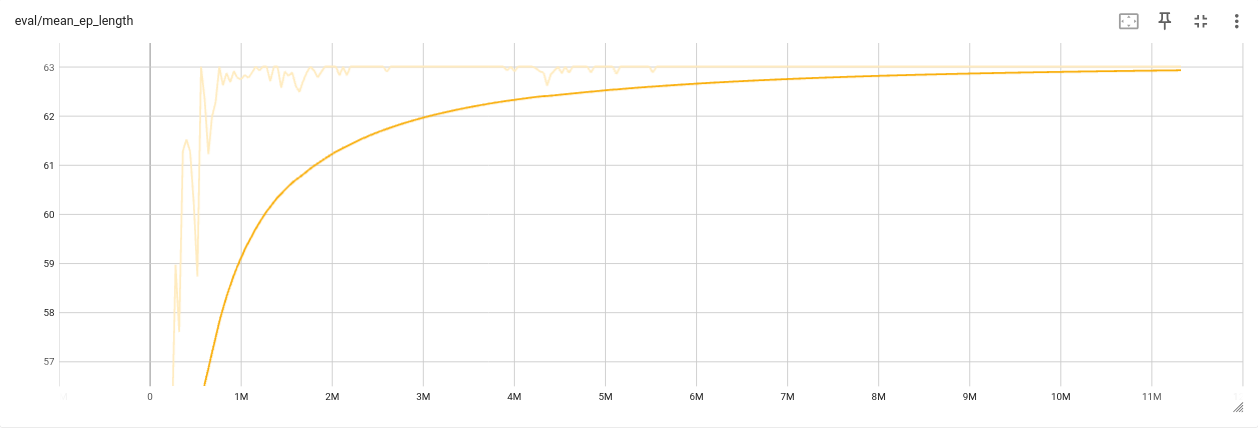
\includegraphics[scale=0.36]{../images/0091 Ende-zu-Ende 1.png}{\\Die mittlere Episodendauer nimmt ab. Das Modell scheint kürzere Updateschrittweiten zu bevorzugen. Welche darüberhinausgehende Bedeutung das Verhalten hat, könnte durch weiterführende Untersuchungen analysiert werden.}
\end{center}
\begin{center}
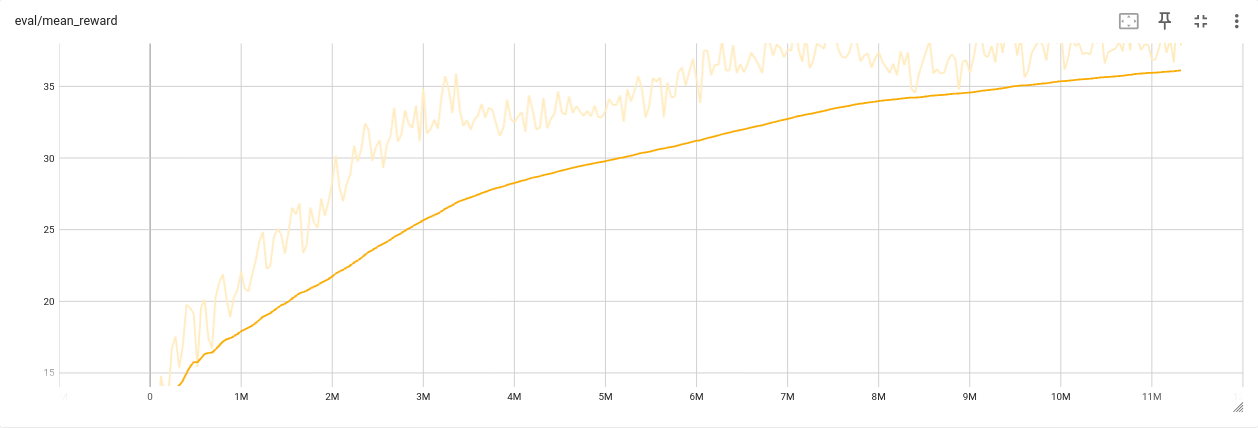
\includegraphics[scale=0.36]{../images/0092 Ende-zu-Ende 2.png}{\\Der Plot zeigt die erste stetig steigende Belohnungskurve eines Ende-zu-Ende-Modells. Ideal wäre, das die mittlere Belohnung der mittleren Episodenlänge entspricht. Doch davon ist das Modell nach 11.2e6 Episoden noch weit entfernt.}
\end{center}
Parallel zum Training mit modellbestimmter Schrittweite wurden die Hyperparameter der Default Ende-zu-Ende Version täglich aktualisiert und neue Modelle antrainiert. Mit folgenden Hyperparametern gelang es ein Modell zu trainieren welches lernte und akzeptabel performte.
\vspace*{0.5cm}
\begin{center}
\begin{tabular}[h]{|c|c|c|c|}
\hline 
Konfigurationsparameter & Wert \\
\hline 
Umweltparameter & \\
Schrittweite $\Delta t_{Modell}$ & 0.001s \\
Episodenende & 1s (1000 Schritte)\\
\hline
Quadtrain & \\
$\alpha$ & 1e-4\\
Parallele Umwelten & 4\\
Batch & 16\\
Netzwerktopologie $\pi$ & [2, 2]\\
Netzwerktopologie $V^{\pi}$ & [2, 2]\\
\hline
Quadendezuende & \\
Aktionsraum & [100$\frac{rad}{s}$\ bis\ 600$\frac{rad}{s}$, $\Delta t_{PPO}$ = $\Delta t_{Modell}$]\\
Belohnungsfunktion & [$\alpha_r$ = 0.0, $\beta_r$ = 0.6, $\gamma_r$ = 0.2, $\delta_r$ = 0.2]\\
\hline
\end{tabular}
\end{center}
\vspace*{0.5cm}
Als Regler kann dieses Modell noch nicht eingesetzt werden, da es insbesondere die Drehlageregelung\\ noch nicht generalisiert hat. Aber zumindest hat das Modell verstanden den 8 Sollgeschwindigkeitsvektoren mehr oder minder zu folgen. Zu erwarten ist, dass durch längeres Training die Güte weiter maximiert werden kann. Ob das tatsächlich der Fall ist, wird Gegenstand zukünftiger Trainings- und Testepochen sein.
\begin{center}
	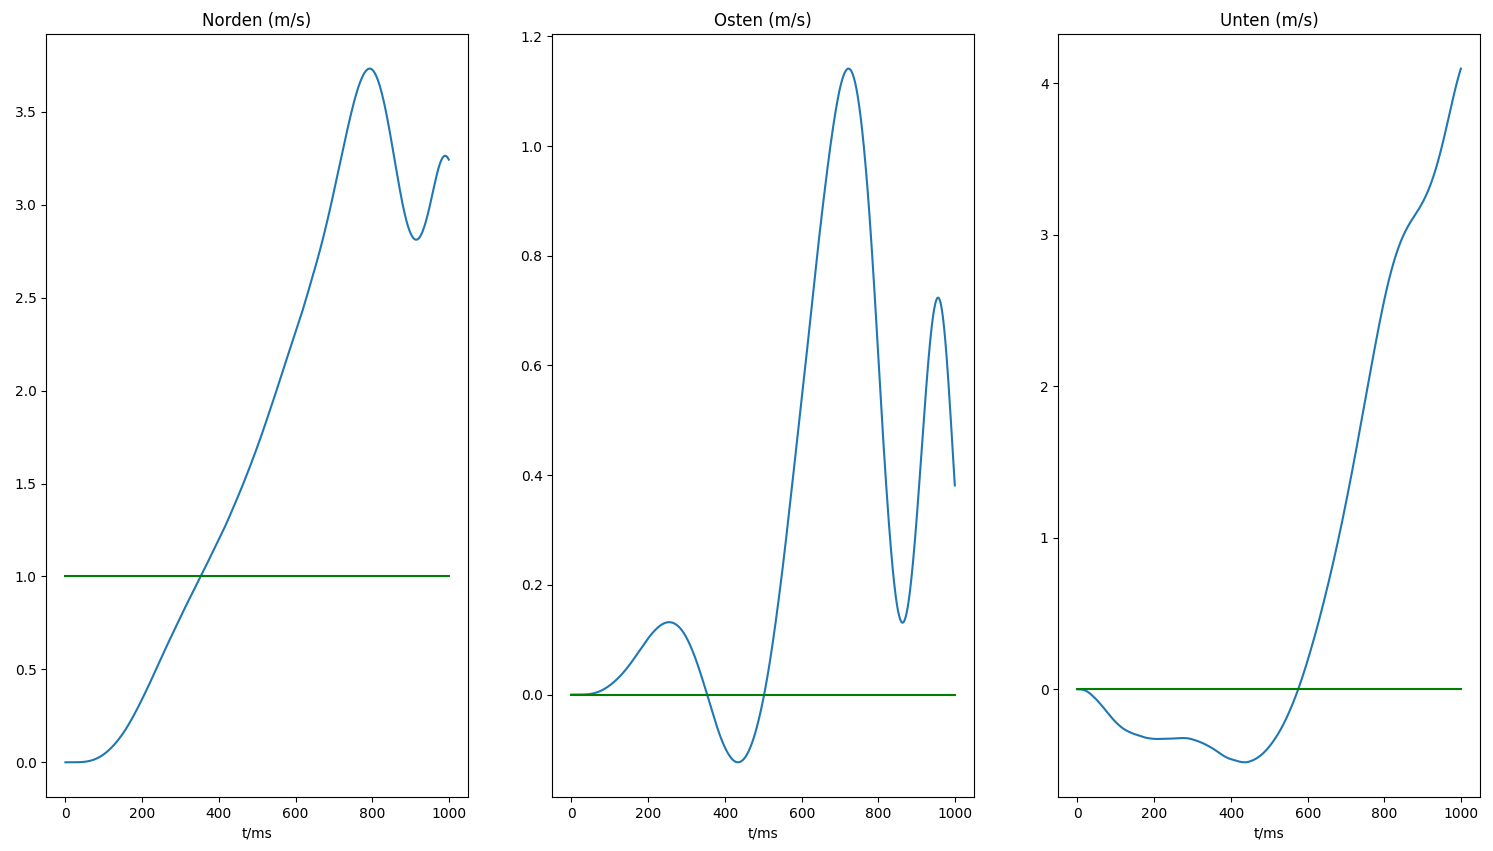
\includegraphics[scale=0.25]{../images/0081 Model E 1.png}{\\Sollgeschwindigkeit nach Norden ist 1 und nach Osten Null. Das Modell regelt den Quadcopter in die korrekte Richtung schwingt aber stark über. Auf den anderen Achsen zeigt das Modell unerwünschtes Verhalten, so driftet der Quadcopter um bis zu 1m und fällt 4m kann sich nach Osten hin aber stabilisieren mit einem erkennbar abnehmenden Fehler.}
\end{center}
\begin{center}
	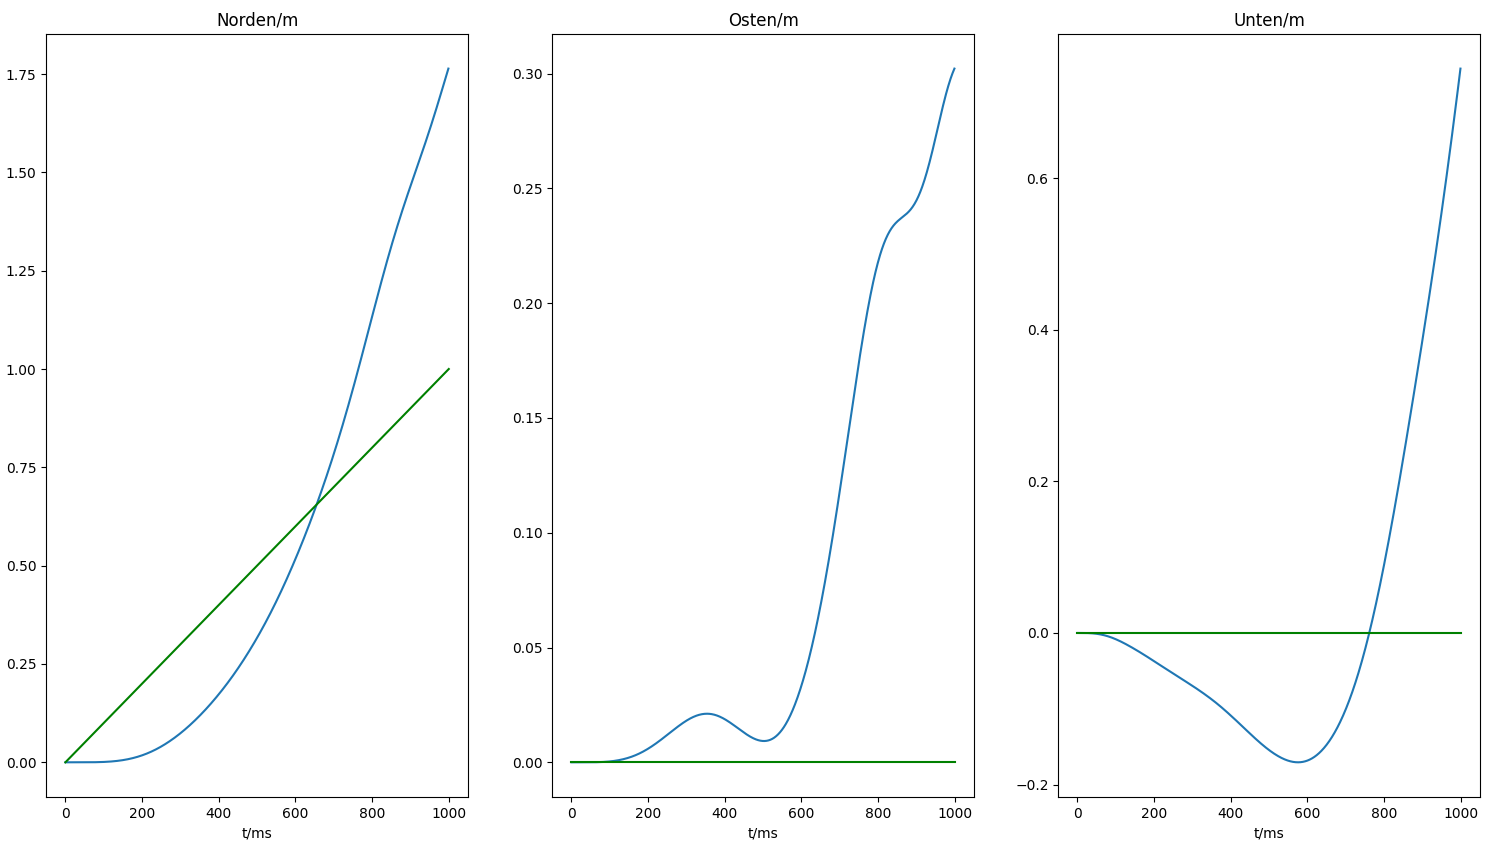
\includegraphics[scale=0.25]{../images/0080 Model E 2.png}{\\Interessant ist zunächst, dass das Integral zwischen der Differenz von der Soll- und Isttrajektorie über den Episodezeitraum von 1s ungefähr Null ist. Womöglich nur Zufall.}
\end{center}
\begin{center}
	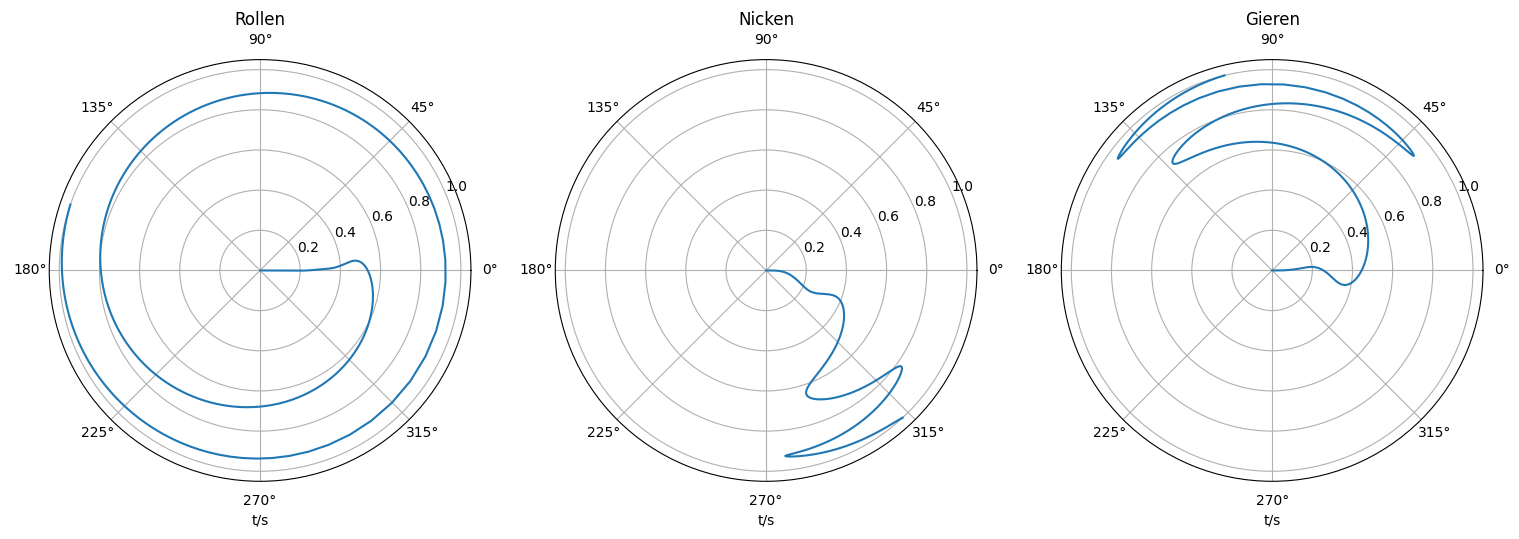
\includegraphics[scale=0.25]{../images/0079 Model E 3.png}{\\Die Drehlagentrajektorien offenbaren das Problem des Ende-zu-Ende-Modells. Nach circa 0.4s verliert es die Kontrolle über die Drehlage.}
\end{center}
Für einen anderen Geschwindigkeitssollvektor welcher nach Süd-Osten zeigt ergeben sich die folgenden Bilder.
\begin{center}
	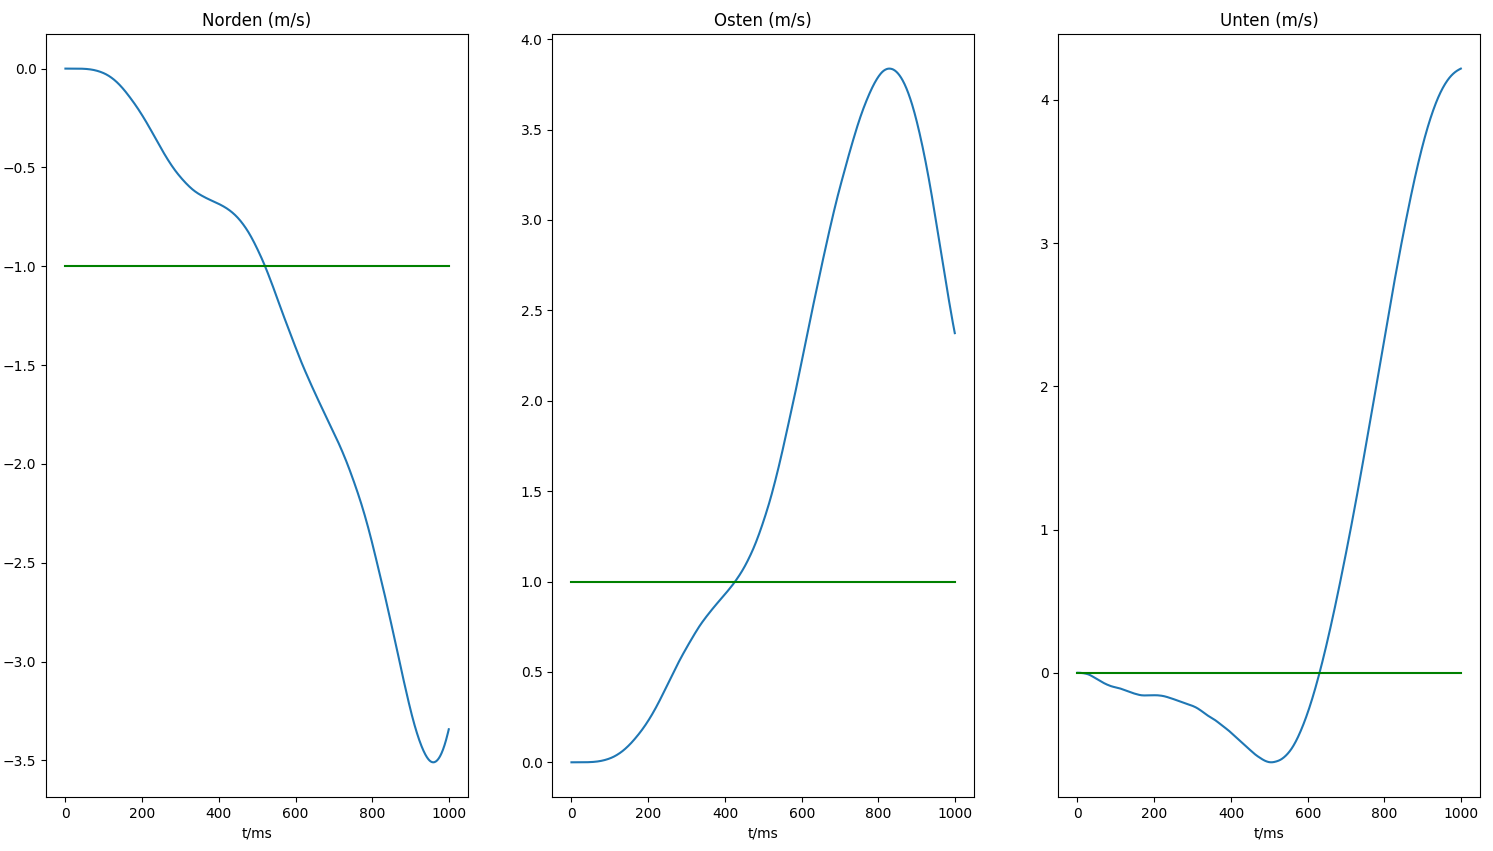
\includegraphics[scale=0.25]{../images/0085 Ende-zu-Ende Nordgeschwindigkeit Ostgeschwindigkeit Untengeschwindigkeit.png}{\\Grundsätzlich ist das Modell in der Lage grob den Sollgeschwindigkeiten zu folgen.}
\end{center}
\begin{center}
	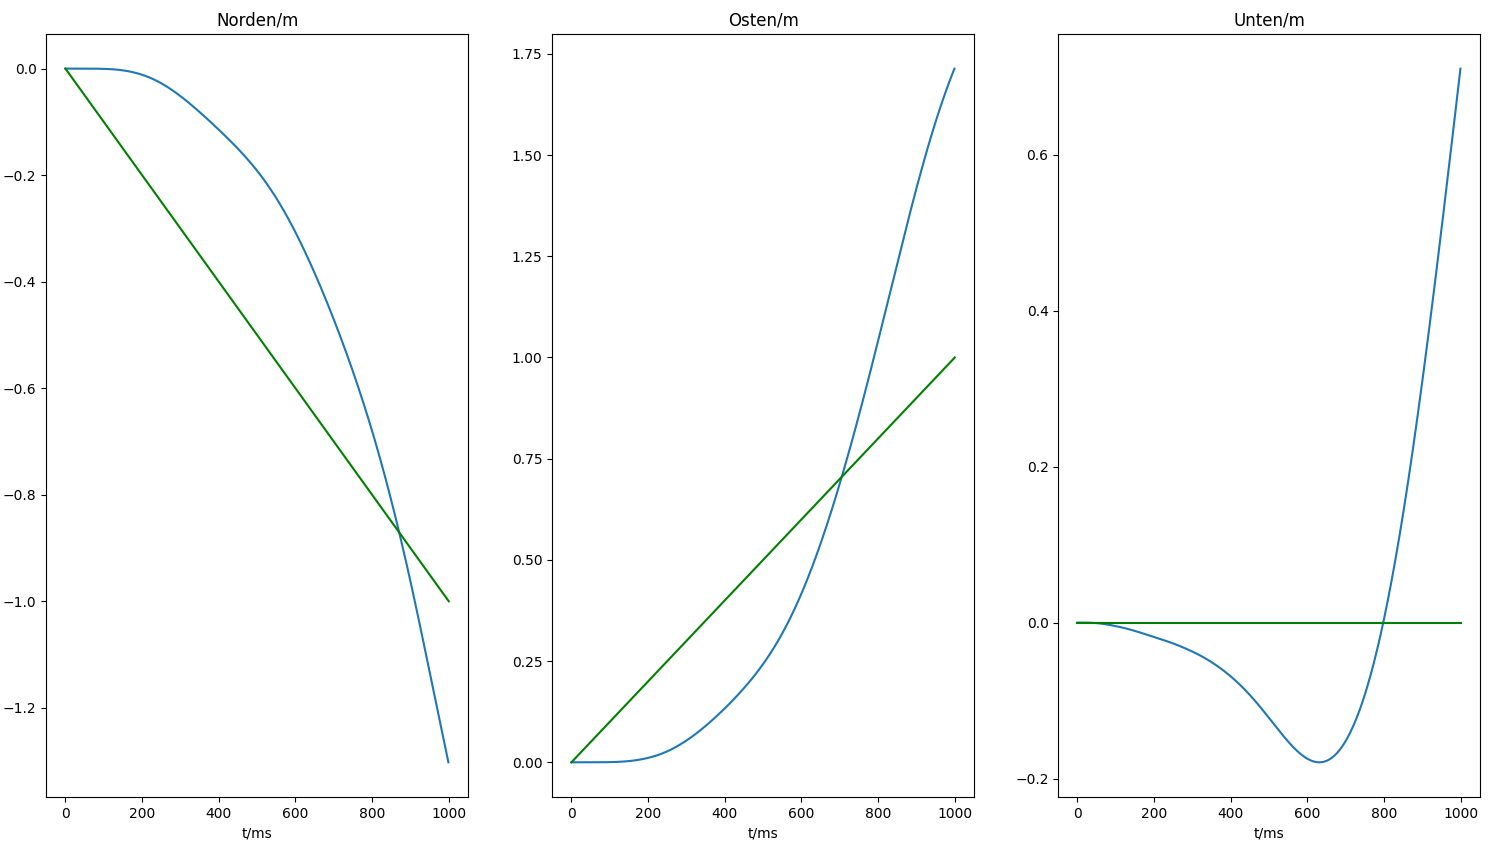
\includegraphics[scale=0.25]{../images/0084 Ende-zu-Ende Nord Ost Unten.png}{\\Die Positionstrajektorien zeigen ein ähnliches Bild wie im vorangegangen Beispiel.}
\end{center}
\begin{center}
	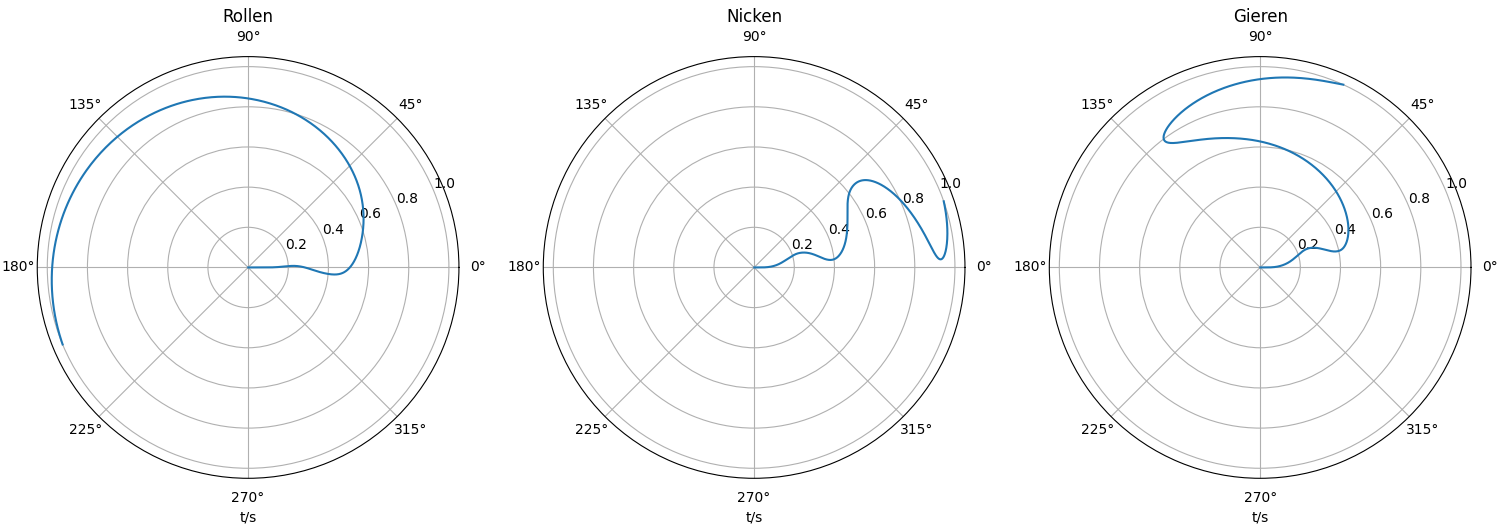
\includegraphics[scale=0.25]{../images/0086 Ende-zu-Ende Rolllage Nickrate Gierrate.png}{\\Auch bei einem anderen Sollgeschwindigkeitsvektor verliert das aktuell beste Modell die Kontrolle über den Quadcopter macht aber auch deutlich, das es die Aufgabe verstanden hat.}
\end{center}

\subsection{\label{Reglerimplementierung:Reglerimplementierung}Implementierung des Reglers}
Die Implementierung des Reglers umfasst alle Implementierungsschritte, die notwendig sind zur Quadcopterzustandsschätzung, zur Berechnung von Reglerbefehlen und für die BLDC-Motorenansteuerung.\\
Für die Programmierung der Informationsflussteilsysteme wurde neben der STM32CubeIDE Entwicklungsumgebung auch Zephyr in Kombination mit Visual Studio Code als Implementierung des Reg Entwicklungsumgebung betrachtet. Nachdem sich der Aufwand für das vollumfängliche Lernen des Zephyr-Devicetrees als zu umfänglich herausgestellt hatte, wurde für die weitere Entwicklung mit der STM32CubeIDE in der Version 1.16.0 gearbeitet.\\
Aus zeitlichen Gründen konnte eine Implementierung des trainierten Modells auf dem Mikrocontroller nicht angegangen geschweige den getestet werden. Dafür wurde der PID-Regler aus \ref{simcon:simcon} adaptiert und portiert auf den STM32F411RE Mikrocontroller. \\
Die vier BLDC-Motoren werden angesteuert über vier unabhängige PWM-Signale welche alle mit Timer 1 generiert werden. Die PWM-Signale liegen auf den Pins PA8, PA9, PA10, und PA11. Aus der Pinkonfiguration ist ersichtlich, dass diesen Pins jeweils ein Timer-Kanal zugeordnet ist. 
\begin{center}
	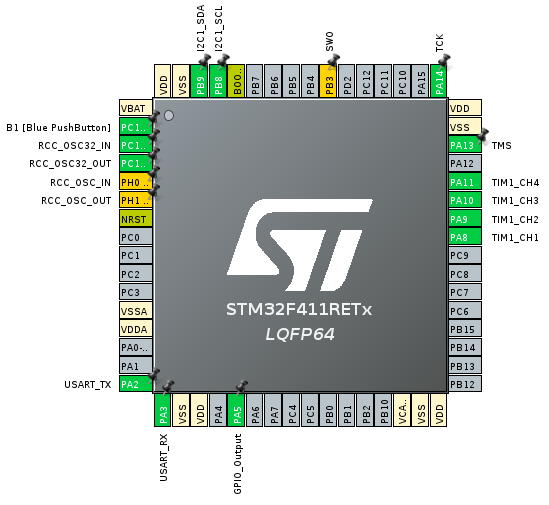
\includegraphics[scale=0.5]{../images/0064 Pinbelegung.png}{\\Pinkonfiguration in der STM32CubeIDE}
\end{center}
Das Pindiagramm wurde herangezogen um die Pins auf dem Board zu lokalisiert. Um die Pins während der Entwicklungsphase schnell zu finden wurden die verwendeten Pins vorsichtig angewinkelt.
\begin{center}
	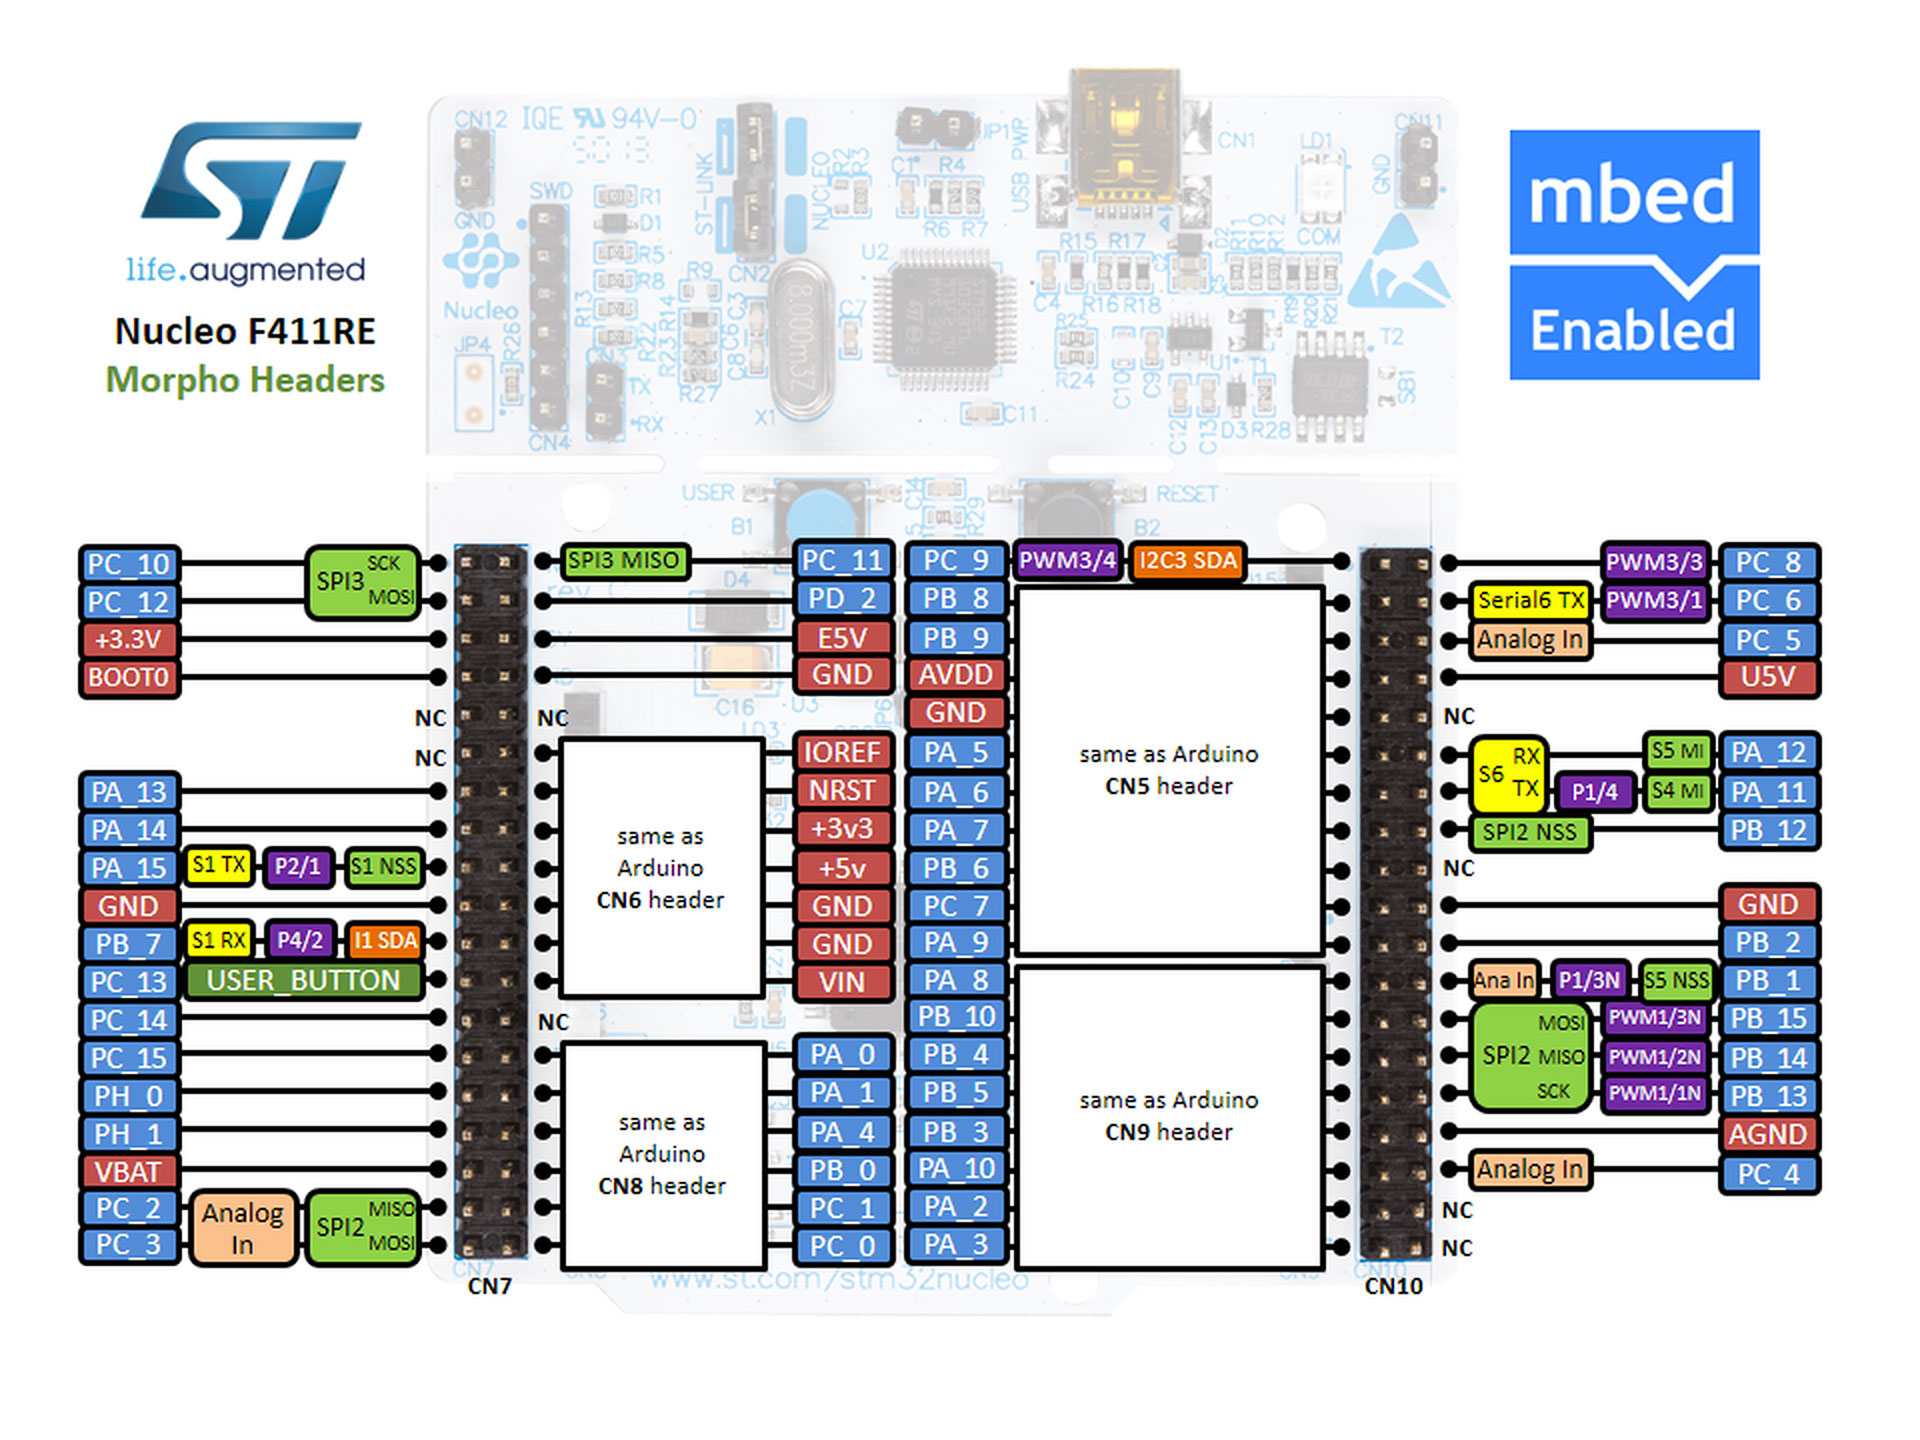
\includegraphics[scale=0.14]{../images/0067 Pinout NUCLEO F411RE.jpeg}{\\Pindiagramm des NUCLEO-F411RE Boards \ref{bild:Pinout}}
\end{center}
Der Duty-Cycle entspricht dem Wert im Capture-Compare-Register (CCR) in welche die Sollwerte direkt geschrieben werden. Die PWM-Frequenz mit welcher die Treiber arbeiten kann zwischen 50Hz und 60Hz liegen \ref{link:Treiberdatenblatt}. Diese wurde mit der System Clock eingestellt. Bei einer Frequenz von 16Mhz wurde ein Prescaler mit Wert 8 und einer Periode von 30259 eingestellt, um circa 60Hz für das PWM-Signal bereitzustellen.
\begin{center}
	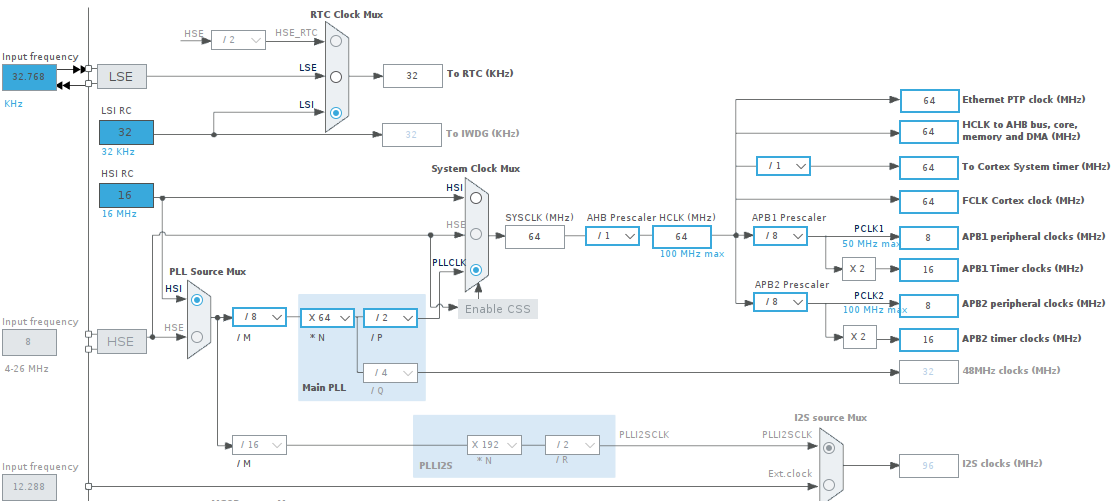
\includegraphics[scale=0.35]{../images/0065 Clock.png}{\\Clock Konfiguration in der STM32CubeIDE}
\end{center}
Mit einer Frequenz von 100Hz wird die Funktion \textit{regelschritt} ausgeführt. Frei wählbar war die Frequenz nicht da es galt sie auf die MotionFX Sensorfusion abzustimmen. Die Funktion \textit{MX\_MEMS\_INIT} initialisiert die Inertiale Messeinheit und konfigurert den Kalmanfilter für die Sensorfusion. 
\begin{center}
\begin{tikzpicture}[font=\sffamily,every label/.append
style={font=\small\sffamily,align=center}]

\node[doc, fill=white] (Quadcontroller) {quadregler.c\\  \begin{lstlisting}[language=C, basicstyle=\fontsize{8}{10}\selectfont]
...
int main(void)
{
	uint16_t timer_val;

	HAL_Init();
	SystemClock_Config();
	MX_GPIO_Init();
	MX_DMA_Init();
	MX_CRC_Init();
	MX_TIM3_Init();
	MX_RTC_Init();
	MX_TIM1_Init();
	MX_TIM2_Init();
	MX_MEMS_Init();
	MX_USART2_UART_Init();

	HAL_TIM_PWM_Start(&htim1, TIM_CHANNEL_1);
	HAL_TIM_PWM_Start(&htim1, TIM_CHANNEL_2);
	HAL_TIM_PWM_Start(&htim1, TIM_CHANNEL_3);
	HAL_TIM_PWM_Start(&htim1, TIM_CHANNEL_4);

	DWT_Start();
	HAL_TIM_Base_Start(&htim2);
	timer_val = __HAL_TIM_GET_COUNTER(&htim2);

	while (1)
	{
		if (__HAL_TIM_GET_COUNTER(&htim2) - timer_val >= 20)
		{
			timer_val = __HAL_TIM_GET_COUNTER(&htim2);
			regelschritt();
		}
	}
}
...
\end{lstlisting}
};
\end{tikzpicture}
\end{center}
Unter anderem wird in dem Prozess die Funktion \textit{MotionFX\_manager\_init} aufgerufen. In dieser kann unter anderem die Orientierung der Sensoren festgelegt werden. Hilfreich war dabei die Dokumention von STMicroelectronics, ganz besonders \ref{link:MotionFX}.
\begin{center}
\begin{tikzpicture}[font=\sffamily,every label/.append
style={font=\small\sffamily,align=center}]

\node[doc, fill=white] (Quadcontroller) {MotionFX\_manager\_init.c\\\begin{lstlisting}[language=C, basicstyle=\fontsize{8}{10}\selectfont]
...
void MotionFX_manager_init(void)
{
	...
	MotionFX_initialize((MFXState_t *) mfxstate);
	MotionFX_getKnobs(mfxstate, ipKnobs);

	ipKnobs->ATime = 1.0;
	ipKnobs->MTime = 8.0;
	ipKnobs->FrTime = 1.0;
	strcpy(ipKnobs->acc_orientation, "NED");
	strcpy(ipKnobs->gyro_orientation, "NED");
	strcpy(ipKnobs->mag_orientation, "NED");
	BSP_SENSOR_ACC_GetOrientation(ipKnobs->acc_orientation);
	BSP_SENSOR_GYR_GetOrientation(ipKnobs->gyro_orientation);
	BSP_SENSOR_MAG_GetOrientation(ipKnobs->mag_orientation);
	ipKnobs->gbias_acc_th_sc = GBIAS_ACC_TH_SC;
	ipKnobs->gbias_gyro_th_sc = GBIAS_GYRO_TH_SC;
	ipKnobs->gbias_mag_th_sc = GBIAS_MAG_TH_SC;
	ipKnobs->output_type = MFX_ENGINE_OUTPUT_NED;
	// Lernmodus
	ipKnobs->LMode = 1;
	...
}
...
\end{lstlisting}
};
\end{tikzpicture}
\end{center}
In der Funktion \textit{regelschritt} werden alle Tasks ausgeführt, welche der Regler hat. Zunächst werden die Sensoren auslesen und mit der Bibliothek MotionFX fusioniert.
\begin{center}
\begin{tikzpicture}[font=\sffamily,every label/.append
style={font=\small\sffamily,align=center}]

\node[doc, fill=white] (Quadcontroller) {quadcontroller.c\\\begin{lstlisting}[language=C, basicstyle=\fontsize{8}{10}\selectfont]
...
void regelschritt(void) {
	// Beschleunigungsensor auslesen mit einer Funktion
	// des X-Cube-MEMS1 Board Support Package
	// BSP_SENSOR_ACC_GetAxes(&AccValue);
	READ_ACCELEROMETER();
	// Gyro auslesen
	// BSP_SENSOR_GYR_GetAxes(&GyrValue);
	READ_GYRO();
	// Magnetometer auslesen
	// BSP_SENSOR_MAG_GetAxes(&MagValue);
	READ_MAG();
	/* Convert angular velocity from [mdeg/s] to [deg/s] */
	// Gieren (Uhrzeigersinn)
	data_in.gyro[0] = (float) GyrValue.x * FROM_MDPS_TO_DPS;
	// Nicken (Nase nach unten ist negatives nicken)
	data_in.gyro[1] = (float) GyrValue.y * FROM_MDPS_TO_DPS;
	// Rollen (Mit Blick von hinten im Uhrzeigersinn)
	data_in.gyro[2] = (float) GyrValue.z * FROM_MDPS_TO_DPS;
	// Norden in g
	data_in.acc[0] = (float) AccValue.x * FROM_MG_TO_G;
	// Osten in g
	data_in.acc[1] = (float) AccValue.y * FROM_MG_TO_G;
	// Oben in g
	data_in.acc[2] = (float) AccValue.z * FROM_MG_TO_G;
	data_in.mag[0] = (float) MagValue.x * FROM_MGAUSS_TO_UT50;
	data_in.mag[1] = (float) MagValue.y * FROM_MGAUSS_TO_UT50;
	data_in.mag[2] = (float) MagValue.z * FROM_MGAUSS_TO_UT50;
	delta_t_s = DWT_Stop() * 1e-6f;
	DWT_Start();
	// Sensorfusion bei 100Hz
	MotionFX_manager_run(fusionin, fusionout, 0.01f);
	...
}
...
\end{lstlisting}
};
\end{tikzpicture}
\end{center}
Eingangswerte für die Fusion wurden vorher in die Struktur \textit{fusionein} geschrieben und Ausgangswerte werden in \textit{fusionout} gespeichert. Diese sind die Lage in Quaternionenform und in Eulerwinkelform, lineare Beschleunigung, der Gravitationsvektor und ein Richtungsfehler. Daraufhin werden die Werte skaliert und zu Gleitkommazahlen umgewandelt, sodass Sie vom Drehlage- und geschwindigkeitsrechner sinnvoll prozessiert werden. Da die linearen Beschleunigungswerte für den Geschwindigkeitsregler einmal integriert werden wird $\Delta t_{PID}$ bestimmt. Auch möglich wäre mit einem Konstanten Wert von 1e-2s zu arbeiten da diese Frequenz im Regelfall vorliegt. Für den Entwicklungszeitraum hat die Messung als robuster erwiesen.
\begin{center}
\begin{tikzpicture}[font=\sffamily,every label/.append
style={font=\small\sffamily,align=center}]

\node[doc, fill=white] (Quadcontroller) {quadcontroller.c\\\begin{lstlisting}[language=C, basicstyle=\fontsize{8}{10}\selectfont]
...
void regelschritt(void) {
	...
	// Setzen der Sollposition mit Joystickwerten
	sollgeschwindigkeit.norden = joystick_nicken / 50.0f;
	sollgeschwindigkeit.osten = joystick_rollen / 50.0f;
	sollgeschwindigkeit.unten = joystick_schub / 50.0f;

	// Integration der Beschleunigungen
	// [m/s]
	geschwindigkeit[NORDEN] += (
		delta_t_s * fusionout->linear_acceleration[SENSOR_NORDEN] / 9.81f
	);
	// [m/s]
	geschwindigkeit[OSTEN] += (
		delta_t_s * fusionout->linear_acceleration[SENSOR_WESTEN] / 9.81f
	);
	// [m/s]
	geschwindigkeit[UNTEN] += (
		delta_t_s * fusionout->linear_acceleration[SENSOR_OBEN] / 9.81f
	);
	drehlage.w = fusionout->quaternion[QW];
	drehlage.x = fusionout->quaternion[QX];
	drehlage.y = fusionout->quaternion[QY];
	drehlage.z = fusionout->quaternion[QZ];
	// Rollwinkel [deg/s]
	drehrate.rollen = (fusionout->rotation[2] - drehlage_tminus1.rollen) / delta_t_s;
	// Nickwinkel [deg/s]
	drehrate.nicken = (fusionout->rotation[1] - drehlage_tminus1.nicken) / delta_t_s;
	// Gierwinkel [deg/s]
	drehrate.gieren = 0.0f * data_in.gyro[0];
	drehlage_tminus1.rollen = fusionout->rotation[2];
	drehlage_tminus1.nicken = fusionout->rotation[1];
	omega_dot.rollen = (drehrate.rollen - drehgeschwindigkeit_tminus1.rollen) / delta_t_s;
	omega_dot.nicken = (drehrate.nicken - drehgeschwindigkeit_tminus1.nicken) / delta_t_s;
	omega_dot.gieren = 0.0f;
	drehgeschwindigkeit_tminus1.rollen = drehrate.rollen;
	drehgeschwindigkeit_tminus1.nicken = drehrate.nicken;
	...
	// Drehlage- und -geschwindigkeitsregler
	...
	// Setzen der PWM-Signale 
	skalar = (pwmoberegrenze - pwmunteregrenze) / 1000.0f;
	// Pin PA8
	TIM1->CCR1 = (
		(
			skalar * schub * ((
				w_cmd[M1] + w_cmd_tminus1[M1]
			) / 2) + pwmunteregrenze
		) / 1000.0f
	) * 30259;
	...
}
...
\end{lstlisting}
};
\end{tikzpicture}
\end{center} 
Neben der Drehlage arbeitet der Geschwindigkeitsregler auch mit der Drehrate und optional der Drehbeschleunigung. Auf die Drehrate wird durch einen Differenzenquotienten der Drehlage, in Eulerwinkelform, geschlossen. Liegen alle Werte als Gleitkommazahlen vor und sind nicht undefiniert berechnet der Drehraten- und -geschwindigkeitsregler die Motorbefehle. Diese werden skaliert und mit einem einfachen Tiefpass beaufschlagt um die Elektronik und Mechanik zu schonen. Der Duty-Cycle muss auf die ganzzahlige Periode des Timers hoch multipliziert werden. Am Oszilloskop wurde die Validität aller Motorsignale geprüft, wofür die Testbench \ref{testbench:testbench} die perfekten Voraussetzungen bot.\\
Mit der Implementierung des Reglers auf dem Mikrocontroller war die Entwicklung aller System für den Quadcopter vorerst abgeschlossen. Das System war damit in einem Zustand der erste operationelle Tests erlaubte.
\begin{center}
	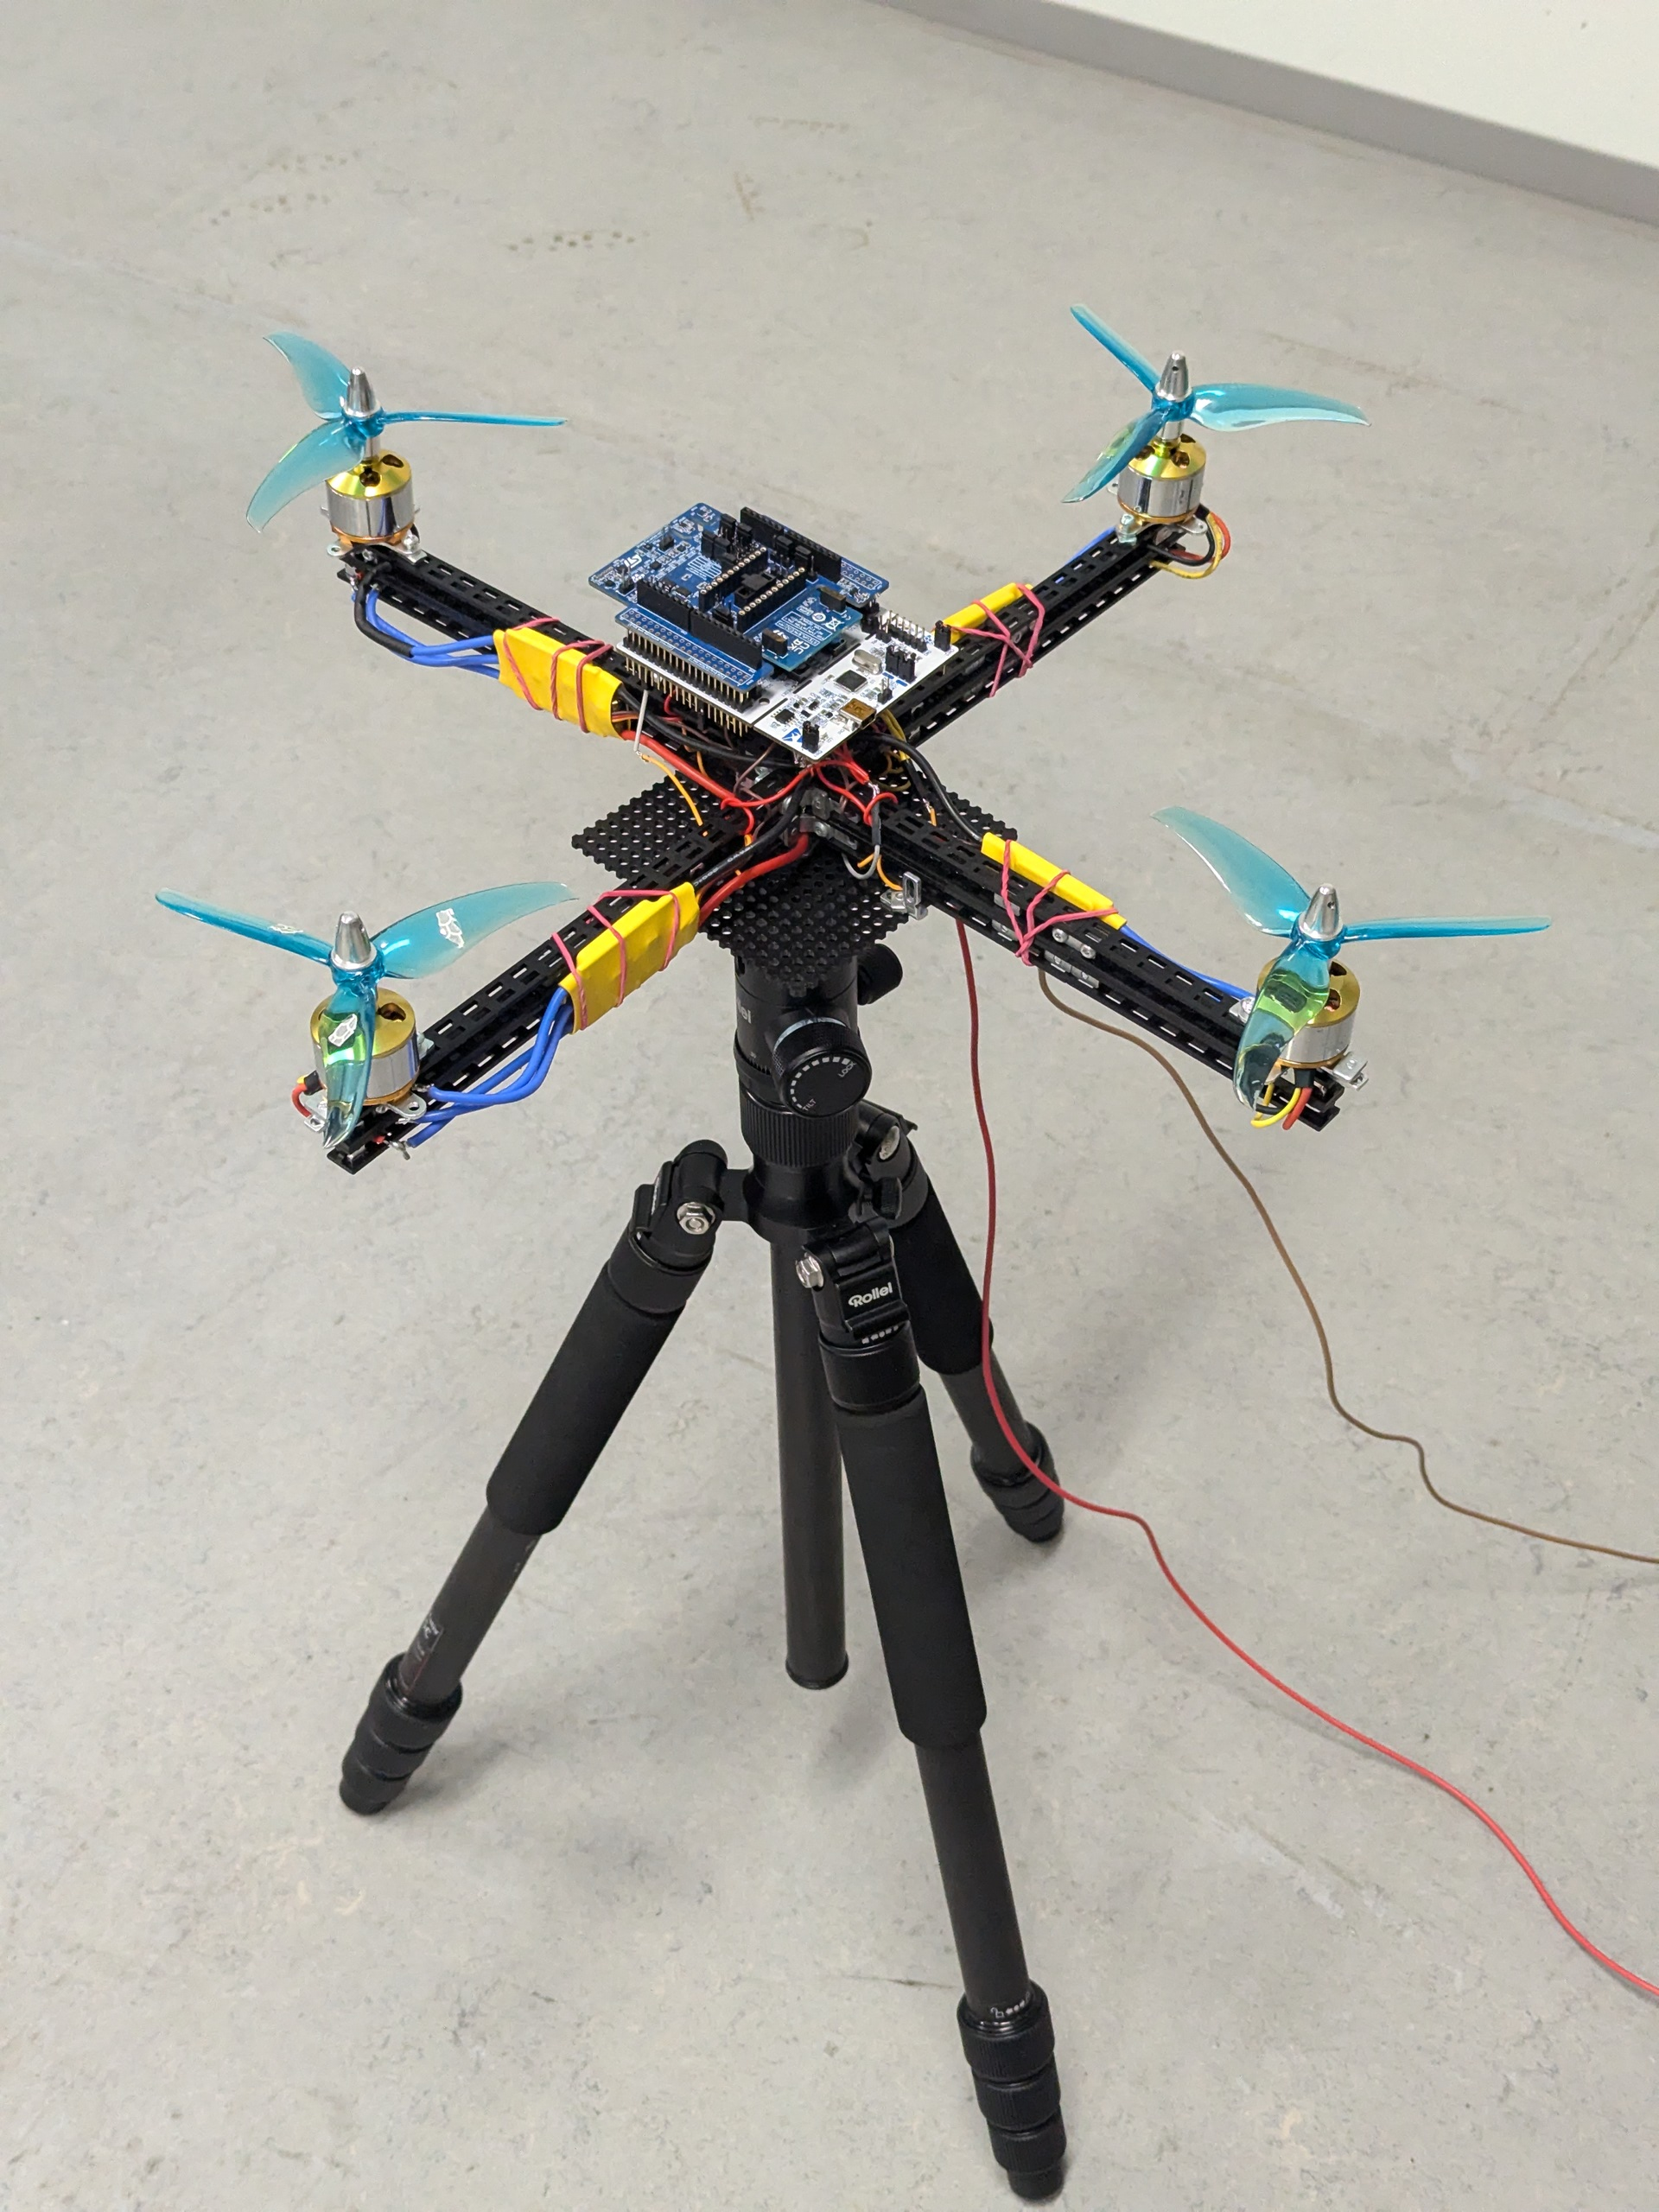
\includegraphics[scale=0.1]{../images/0070 Modell 1.jpg}{\\Prototyp 1 montiert auf einem Kamerastativ}
\end{center}


\subsection{\label{testbench:testbench}Produktion der Testbench}
Die Testbench umfasst, ein Sollwertinterface, die Visualisierung des Quadcopterzustands mittels Flask und ThreeJS sowie das Stativ, auf welchem der Quadcopter befestigt wird, mit Leistung aus einer Spannungsquelle versorgt wird und dessen Signale mit einem Oszilloskop analysiert und aufgezeichnet werden. Das Joystick-Sollwertinterface sampelt den Zustand eines Joysticks mit dem Programm \textit{joystick.py} und sendet den Schubwert und die Lage an die serielle Schnittstelle des NUCLEO-F411RE Board welche aus den Daten eine Sollgeschwindigkeit für den Regler berechnet. Die Samplefrequenz ist Default auf 30Hz eingestellt. Im Gegensatz zum Sollwertinterface welches für das Training der Agenten eingesetzt wurde tangiert das Sollwertinterface nun nicht mehr nur Informationsflussteilsysteme.
Das Pythonprogramm \textit{joystick.py} nutzt die Funktionalitäten der Bibliothek Pygame, wodurch viele verschiedene Joysticks unterstützt werden.\\
\begin{center}
	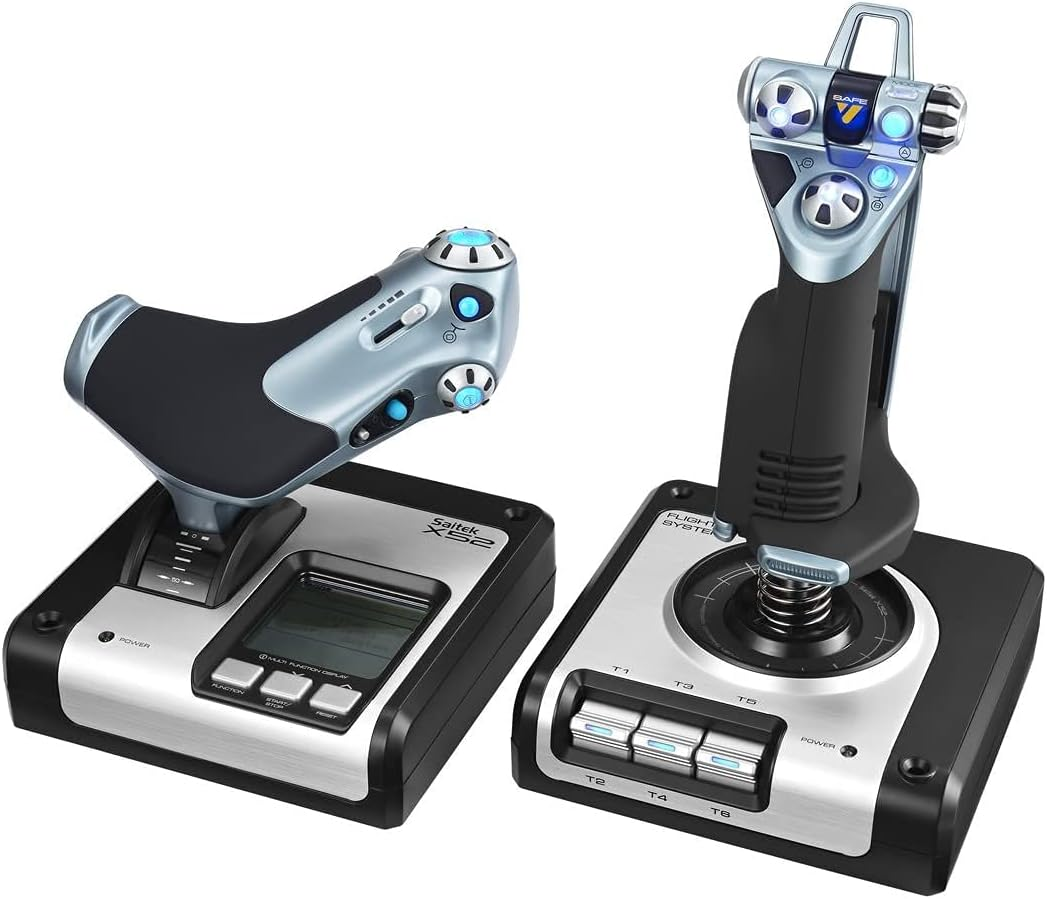
\includegraphics[scale=0.125]{../images/0063 Joystick.jpg
	}{\\Eingesetzter Joystick Saitek X52 \ref{bild:4}}
\end{center}
Der Joystickzustand wird, wenn sich ein Wert ändert, an \textit{quadseriell.py} weitergeleitet und mit der Bibliothek \textit{pyserial} an den Quadcopter gesendet. Der UART-Callback wurde erweitert, um die Joystickbefehle zu prozessieren. Die Befehle für die Nick-, Rollrichtung und den Schub werden auf Intervalle modelliert in welchen alle Werte dreistellig sind. Dadurch wird die Eindeutigkeit der Stellen sichergestellt. Im Callback werden die Werte extrahiert, zurück moduliert und in globale Variablen geschrieben. Am Joystick kann mit einem Radregler welcher visuelles Feedback gibt ein Modus selektiert werden.
\begin{center}
	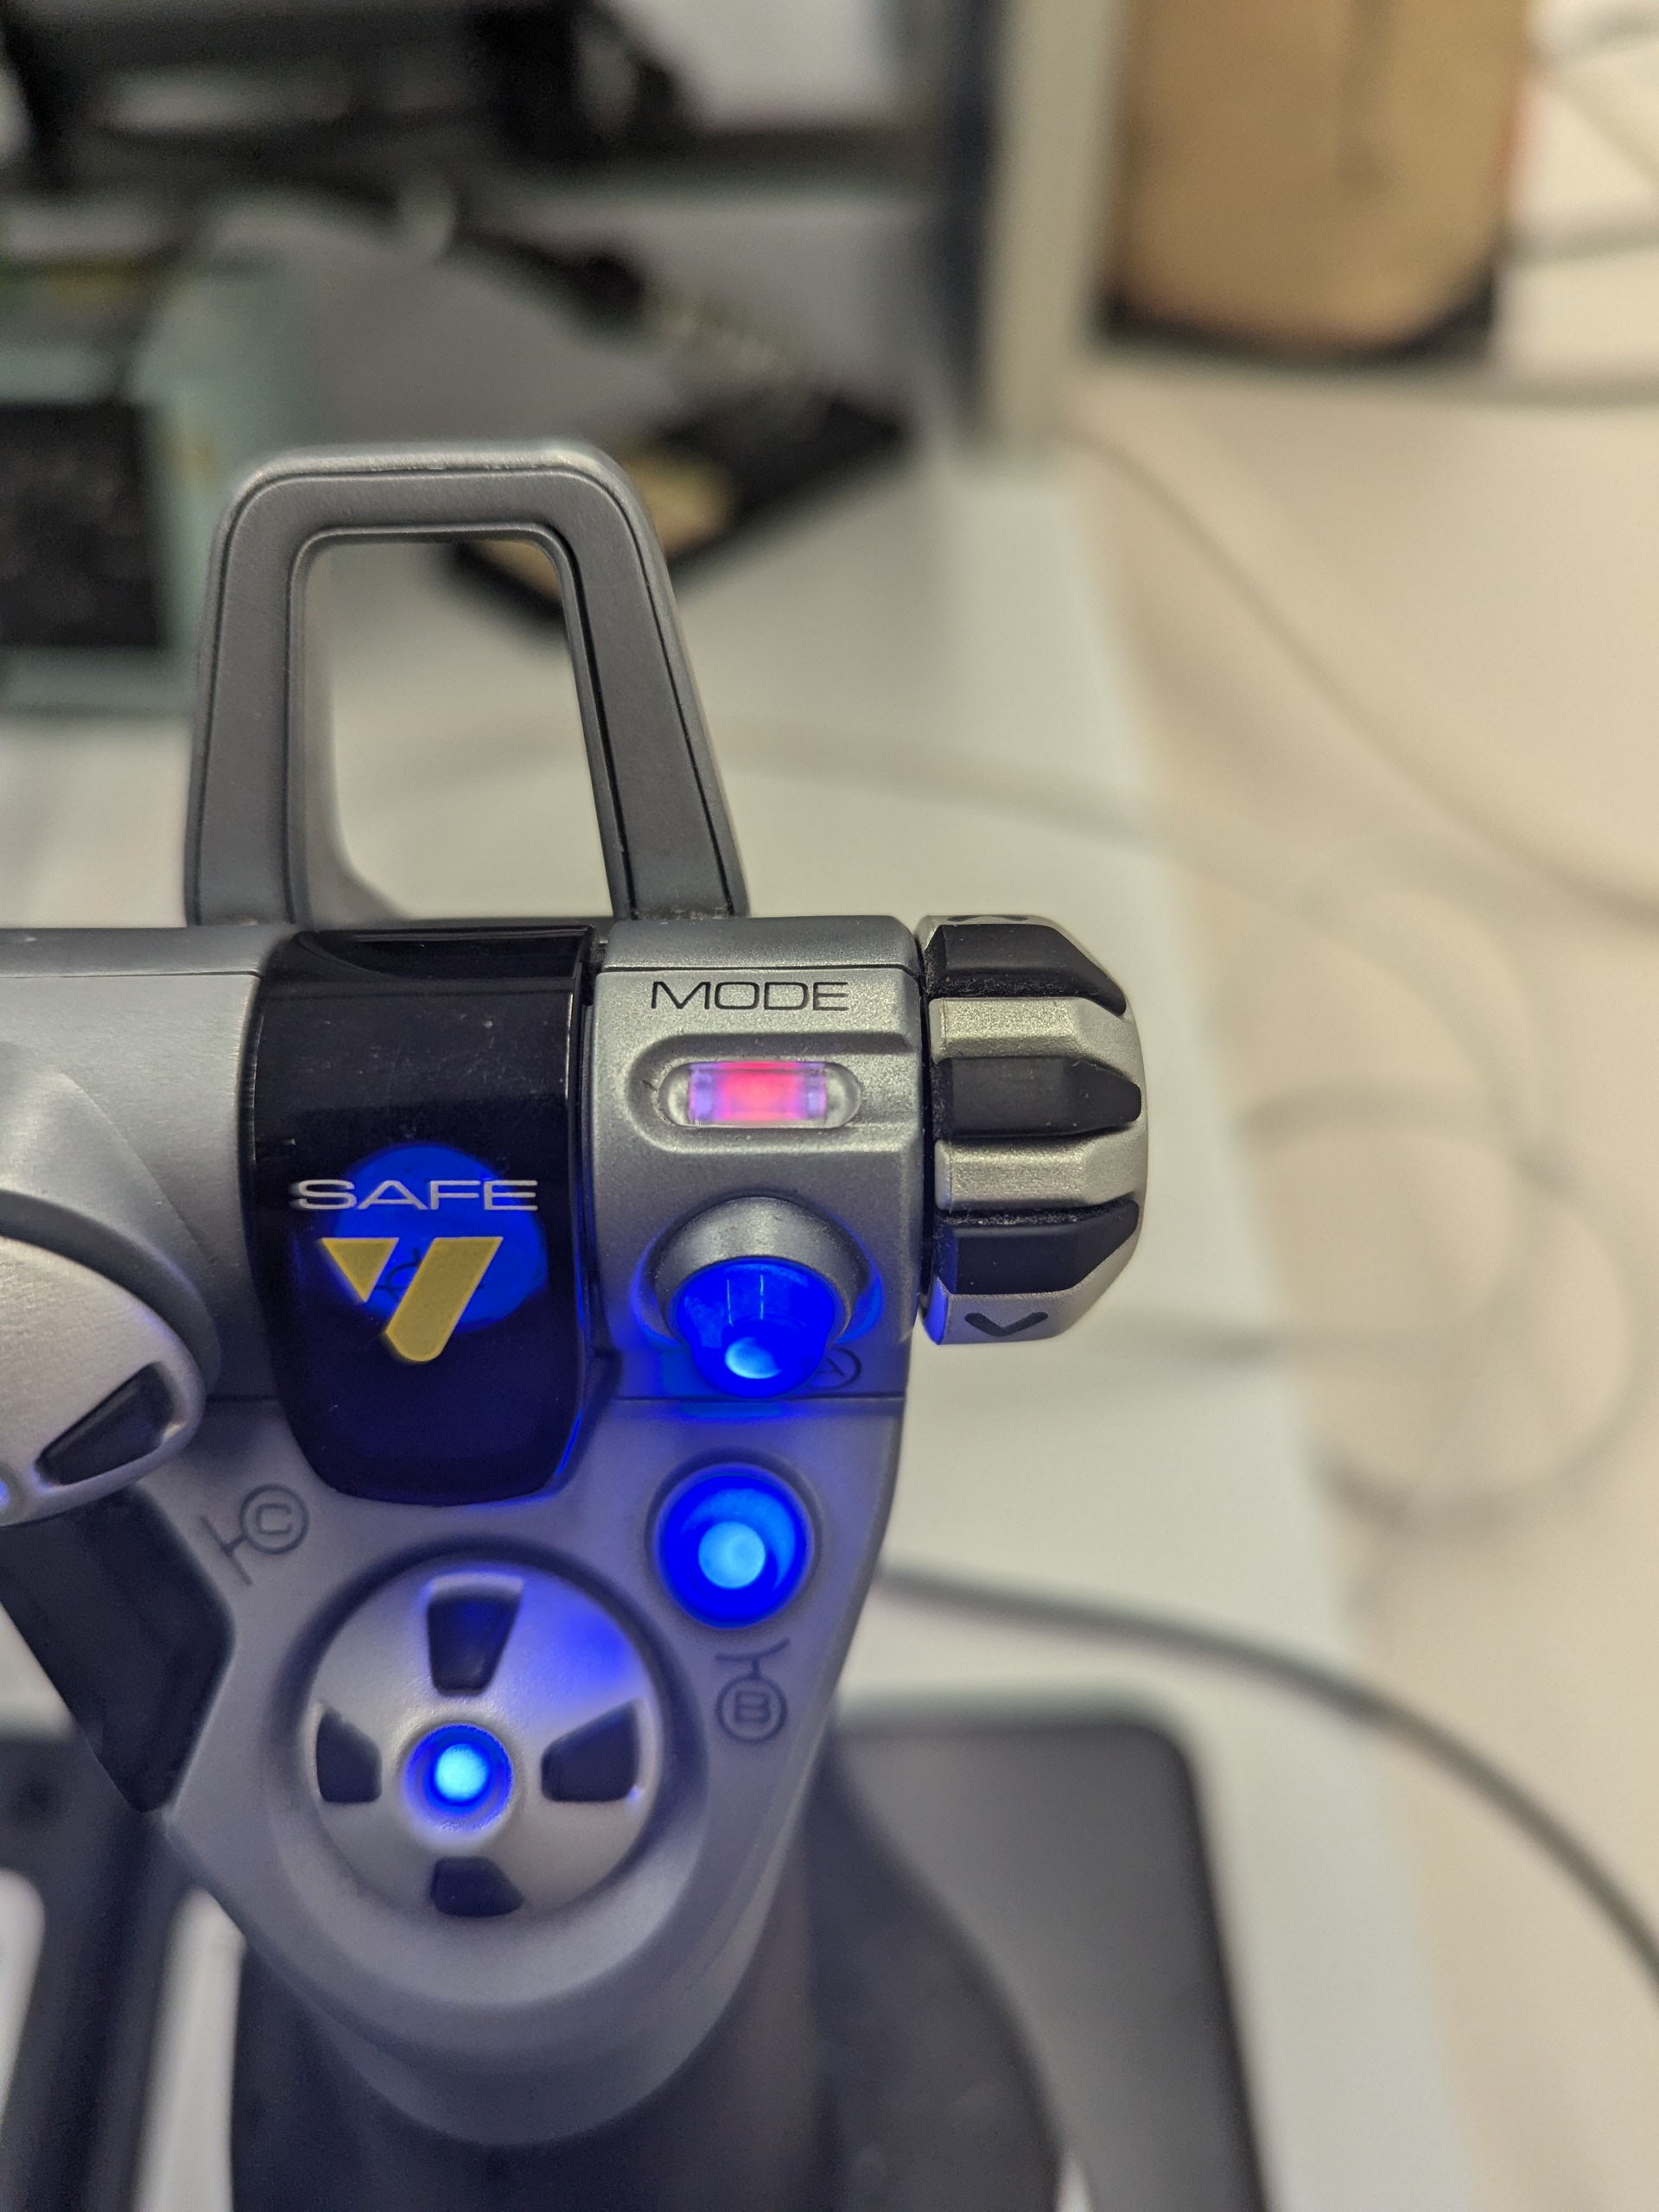
\includegraphics[scale=0.08]{../images/0088 Joystick Mode.jpg}{\\Modus 1 am Joystick ist eingestellt und die LED leuchtet leicht rot.}
\end{center}
Im Modus 0 haben Änderungen am Joystick keinen Effekt auf den Quadcopter. Im Modus 1 entspricht der Joystickschubprozentsatz direkt dem Duty-Cycle wodurch die Drehzahlregler und BLDC-Motoren getestet und programmiert werden können. Der Regler wird aktiv, wenn der Nutzer in Modus 2 wechselt.
\begin{center} 
\begin{tikzpicture}[font=\sffamily,every label/.append
style={font=\small\sffamily,align=center}]

\node[doc, fill=white] (Quadcontroller) {quadcontroller.c\\  \begin{lstlisting}[language=C, basicstyle=\fontsize{8}{10}\selectfont]
...
void USART_CharReception_Callback(void)
{
	/* Auslesen des Zeichens. */
	__IO uint32_t received_char = LL_USART_ReceiveData8(USARTx_INSTANCE);

	if (received_char == '\r') {
		rx_index = 0;
		joystick_schub = (
			100 * ((rx_buffer[0] - '0') - 1) + 
			10 * (rx_buffer[1] - '0') + 
			(rx_buffer[2] - '0')
		);
		if (joystick_schub < 5.0f) {
			regleran = 0;
		} else {
			regleran = 1;
		}
		joystick_nicken = (
			100 * rx_buffer[3] + 10 * rx_buffer[4] + rx_buffer[5] - 500
		);
		joystick_rollen = (
			100 * rx_buffer[6] + 10 * rx_buffer[7] + rx_buffer[8] - 500
		);
		modus2 = rx_buffer[9];
	  	modus1 = rx_buffer[10];
	} else {
		rx_buffer[rx_index] = received_char - '0';
		rx_index += 1;
	}
}
...
\end{lstlisting}
};
\end{tikzpicture}
\end{center}
Die Stromversorgung des Quadcopters wird auf der Testbench mit Kabel sichergestellt welche an ein Netzteil oder einen Lithium-Polymer-Akkumulator geklemmt werden können.\\
Im Modellbaubereich werden Akkus standardisiert nach der Anzahl der in Serie geschalteten Standardzellen. Eine Standardzelle hat 3.7V und wird als S1 bezeichnet. Für den Quadcopter wurde sowohl mit 7.4V als auch mit 11.1V gearbeitet, also mit S2 und S3 Akkus. Wichtig ist einen Kondensator parallel zur Spannungsquelle zu schalten um die Gleichspannung zu stabilieren und auf diese Weise die Elektronik vor Spannungsprüngen und Störrauschen zu 
schützen.
\begin{center}
	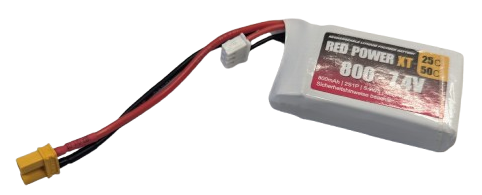
\includegraphics[scale=0.42]{../images/0082 S2 Akku.png}{\\\label{Akku}S2 Akkumulator welcher als Alternativ zu einem Netzteil verwendet werden kann}
\end{center}
Die Montierung des Quadcopters auf einem Kamerastativ war nützlich. Mit leichten Modifikationen und Bauteilen aus dem \textit{Totem} Bausatz konnte der Quadcopter sicher fixiert werden auch ohne festgeschraubt werden zu müssen.
\begin{center}
	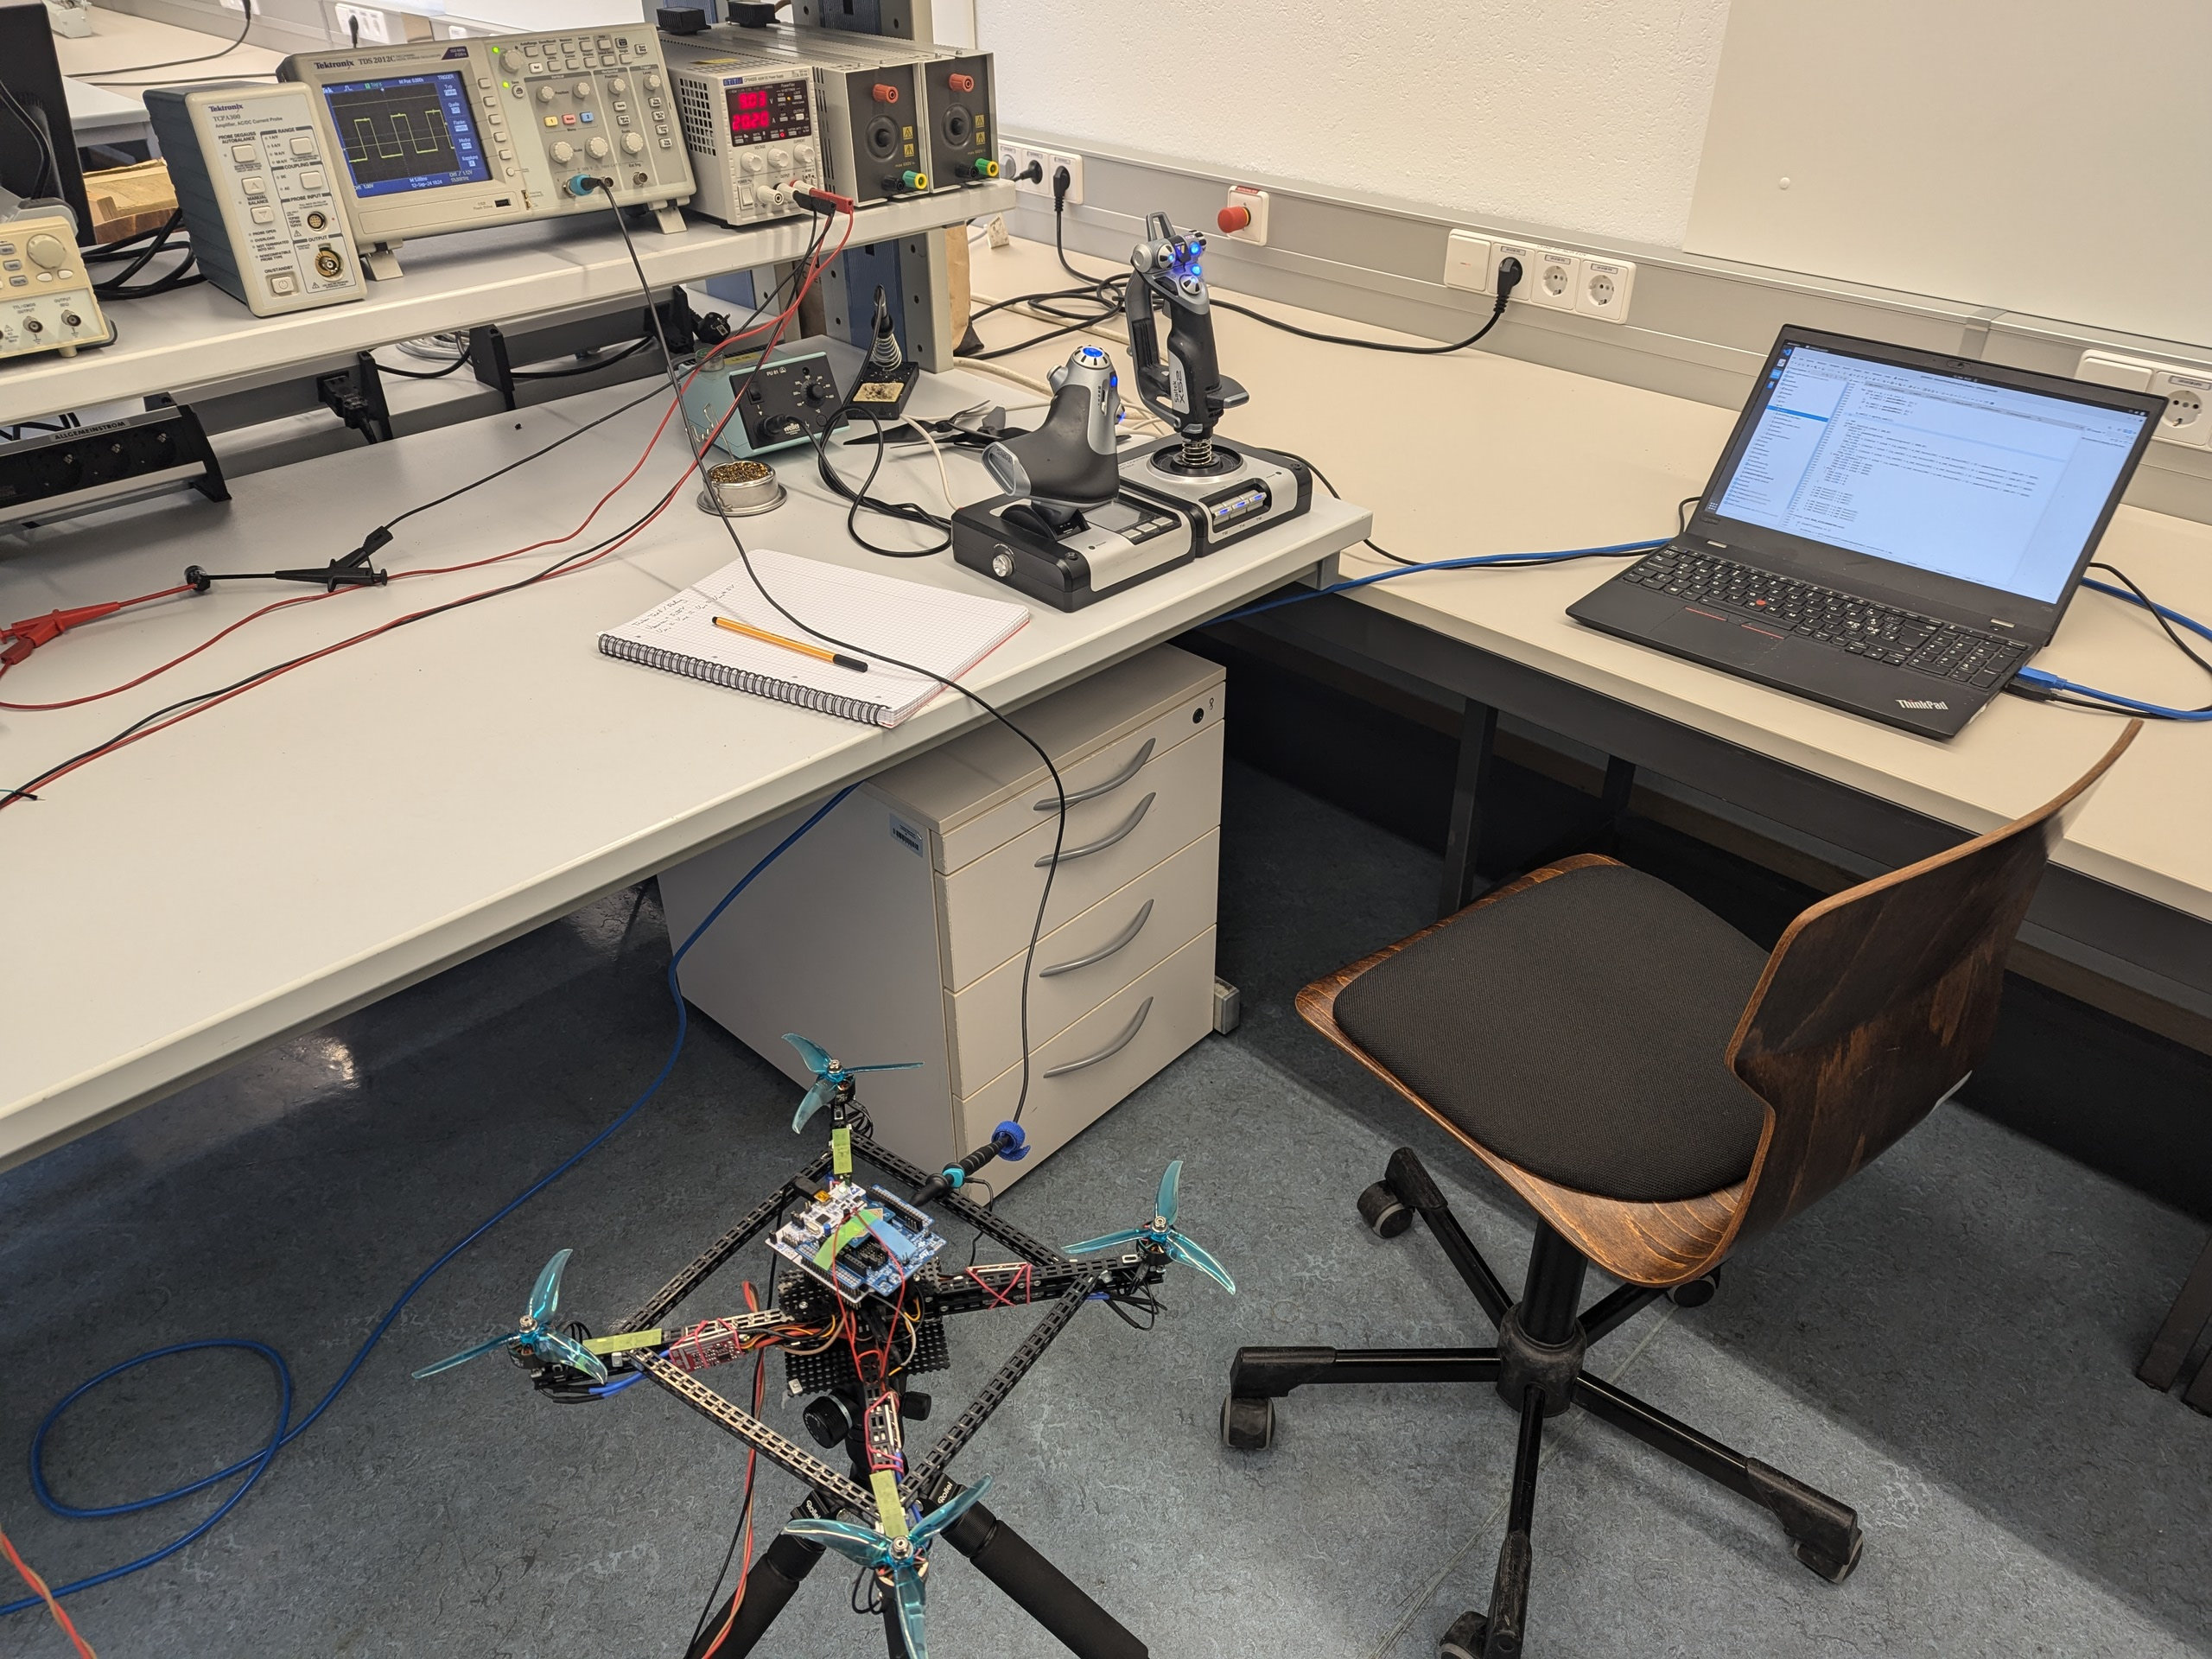
\includegraphics[scale=0.18]{../images/0087 Testbench.jpg}{\\Prototyp 2 montiert auf dem Stativ mit dem Testsetup im Hintergrund}
\end{center}

\subsection{Adaption}
Der Adaptionsteilprozess enthält alle Arbeitsschritte die anfallen, wenn ein neues Teilziel definiert wird oder ein Ziel abgeändert wird. Beispielsweise wurden neue BLDC-Motoren beschafft da die ursprünglich vorgesehenen nicht die gewünschte Drehzahl erreichten. Der Beschaffungsprozess musste also adaptiert werden. Der Adaptionsteilprozess bezieht sich immer auf mindestens einen anderen Teilprozess.\\
Auch Teil der Adaptionsphase waren erste vorsichtige Flugtests welche zur Evaluation und Optimierung des Reglers ausgewertet wurden.
\begin{center}
	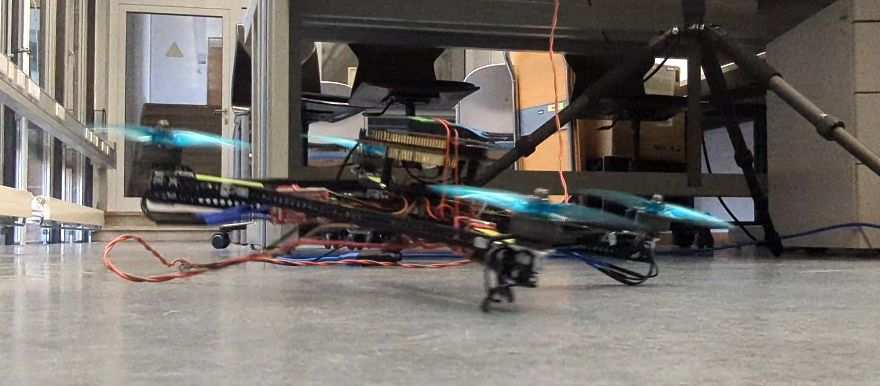
\includegraphics[scale=0.4]{../images/0073 Flugtest.png}{\\Flugtest mit PID-Regler und Joysticksollwertinterface mit Schräglage gleich nach dem Start.}
\end{center}
\begin{center}
	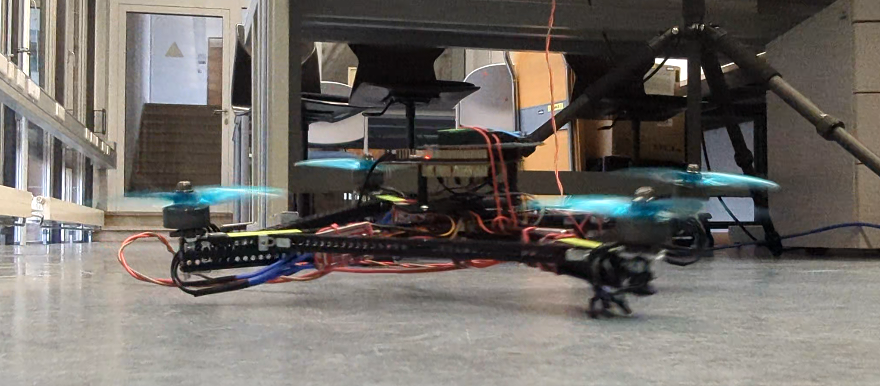
\includegraphics[scale=0.4]{../images/0074 Flugtest.png}{\\Weiterer Flugtest mit PID-Regler und Joysticksollwertinterface bei dem der Quadcopter sich auch schnell zur Seite neigt und instabil wird. Auch ein Gegensteuern am Joystick zeigt kaum Wirkung.}
\end{center}
\begin{center}
	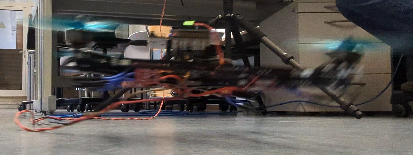
\includegraphics[scale=0.85]{../images/0075 Flugtest.png}{\\Der Quadcopter gewinnt an Höhe doch wird kurz darauf instabil.}
\end{center}
Im aktuellen Zustand geht es bei den Flugtests vor allem darum, den Regler zu debuggen und geeignete PID- und Sensorfusionsparameter zu testen. Die ersten Fehlversuche des Quadcopters wurden noch nicht ausreichend untersucht um abschließend festhalten zu können, warum der Quadcopter schnell instabil wird. Sehr wahrscheinlich ist, dass sich einer der Drehzahlregler kurz nach dem Start ausschaltet. Hinweise dafür ist ein Ton der wenige Sekunden nach dem Abheben zu hören ist und die Tatsache das einer der BLDC-Motoren in einem anderen Duty-Cycle Bereich aktiv wird beim Hochfahren. Möglich ist das der Drehzahlregler defekt oder falsch programmiert ist. Unwahrscheinlicher ist ein Fehler im Regler selbst da dieser in Test die richtigen Motorbefehle demonstrierte und das statische Verhalten der BLDC-Motoren einen korrekten Eindruck macht. Auch nicht auszuschließen ist, dass der Kalman-Filter durch die Eigenschwingungen des Quadcopters gestört wird. Maßnahmen zur Schwingungsminimierung wurden getroffen mit einem verstärkten Rahmen und gefederter Lagerung des Mikrocontrollers sind aber potenziell unzulänglich.\\
Im letzten Implementierung- beziehungsweise Adaptionsschritt wurden alle Software-, Hardwarekomponenten und die Dokumentation auf das wesentliche reduziert, getestet, validiert und geprüft.
Ziel dabei war das Gesamtsystem in einen Zustand zu bringen der zukünftigen Arbeiten so einfach wie möglich macht. Das Problem dabei ist, dass zukünftige Anforderung unbekannt sind. Nichtsdestotrotz lohnt es sich immer auf Nutzerfreundlichkeit zu achten.